\documentclass[hidelinks,12pt]{article}
\usepackage[left=0.25cm,top=1cm,right=0.25cm,bottom=1cm]{geometry}
%\usepackage[landscape]{geometry}
\textwidth = 20cm
\hoffset = -1cm
\usepackage[utf8]{inputenc}
\usepackage[spanish,es-tabla]{babel}
\usepackage[autostyle,spanish=mexican]{csquotes}
\usepackage[tbtags]{amsmath}
\usepackage{nccmath}
\usepackage{amsthm}
\usepackage{amssymb}
\usepackage{mathrsfs}
\usepackage{graphicx}
\usepackage{subfig}
\usepackage{standalone}
\usepackage[outdir=./Imagenes/]{epstopdf}
\usepackage{siunitx}
\usepackage{physics}
\usepackage{color}
\usepackage{float}
\usepackage{hyperref}
\usepackage{multicol}
%\usepackage{milista}
\usepackage{anyfontsize}
\usepackage{anysize}
%\usepackage{enumerate}
\usepackage[shortlabels]{enumitem}
\usepackage{capt-of}
\usepackage{bm}
\usepackage{relsize}
\usepackage{placeins}
\usepackage{empheq}
\usepackage{cancel}
\usepackage{wrapfig}
\usepackage[flushleft]{threeparttable}
\usepackage{makecell}
\usepackage{fancyhdr}
\usepackage{tikz}
\usepackage{bigints}
\usepackage{scalerel}
\usepackage{pgfplots}
\usepackage{pdflscape}
\pgfplotsset{compat=1.16}
\spanishdecimal{.}
\renewcommand{\baselinestretch}{1.5} 
\renewcommand\labelenumii{\theenumi.{\arabic{enumii}})}
\newcommand{\ptilde}[1]{\ensuremath{{#1}^{\prime}}}
\newcommand{\stilde}[1]{\ensuremath{{#1}^{\prime \prime}}}
\newcommand{\ttilde}[1]{\ensuremath{{#1}^{\prime \prime \prime}}}
\newcommand{\ntilde}[2]{\ensuremath{{#1}^{(#2)}}}

\newtheorem{defi}{{\it Definición}}[section]
\newtheorem{teo}{{\it Teorema}}[section]
\newtheorem{ejemplo}{{\it Ejemplo}}[section]
\newtheorem{propiedad}{{\it Propiedad}}[section]
\newtheorem{lema}{{\it Lema}}[section]
\newtheorem{cor}{Corolario}
\newtheorem{ejer}{Ejercicio}[section]

\newlist{milista}{enumerate}{2}
\setlist[milista,1]{label=\arabic*)}
\setlist[milista,2]{label=\arabic{milistai}.\arabic*)}
\newlength{\depthofsumsign}
\setlength{\depthofsumsign}{\depthof{$\sum$}}
\newcommand{\nsum}[1][1.4]{% only for \displaystyle
    \mathop{%
        \raisebox
            {-#1\depthofsumsign+1\depthofsumsign}
            {\scalebox
                {#1}
                {$\displaystyle\sum$}%
            }
    }
}
\def\scaleint#1{\vcenter{\hbox{\scaleto[3ex]{\displaystyle\int}{#1}}}}
\def\bs{\mkern-12mu}


\title{El átomo de hidrógeno} \vspace{-3ex}
\author{M. en C. Gustavo Contreras Mayén}
\date{ }
\newcommand{\Cancel}[2][black]{{\color{#1}\cancel{\color{black}#2}}}
\begin{document}
\vspace{-4cm}
\maketitle
\fontsize{14}{14}\selectfont
\tableofcontents
\newpage

\section{Ecuación de Schrödinger.}
\subsection{Planteamiento inicial.}

La ecuación de Schrödinger es:
\begin{align}
i \, \hbar \, \pdv{\Psi}{t} = H \, \Psi
\label{eq:ecuacion_04_01}
\end{align}

donde el operador Hamiltoniano se obtiene de la energía clásica:
\begin{align*}
\dfrac{1}{2} m \, v^{2} + V = \dfrac{1}{2 \, m} \big( p_{x}^{2} + p_{y}^{2} + p_{z}^{2} \big)
\end{align*}

donde la componente del operador momento es:
\begin{align}
p_{x} \to \dfrac{\hbar}{i} \pdv{x}, \hspace{1cm} p_{y} \to \dfrac{\hbar}{i} \pdv{y}, \hspace{1cm} p_{z} \to \dfrac{\hbar}{i} \pdv{z}
\label{eq:ecuacion_04_02}
\end{align}

o de manera equivalente:
\begin{align}
\vb{p} \to \dfrac{\hbar}{i} \nabla
\end{align}

Entonces la ecuación de Schrödinger resulta:
\begin{align}
i \, \hbar \, \pdv{\Psi}{t} = -\dfrac{\hbar^{2}}{2 \, m} \, \Psi + V \, \Psi
\label{eq:ecuacion_04_04}    
\end{align}

donde $\laplacian$ es el operador Laplaciano en coordenadas cartesianas.

La energía potencial $V$ y la función de onda $\Psi$ son ahora funciones de $\vb{r}(x, y, z)$ y $t$. La probabilidad de encontrar a una partícula en un volumen infinitesimal $\dd[3]{\vb{r}} = \dd{x} \dd{y} \dd{z}$ es $\abs{\Psi(\vb{r}, t)}^{2} \dd[3]{\vb{r}}$ y la condición de normalización es:
\begin{align}
\int \abs{\Psi}^{2} \dd[3]{\vb{r}} = 1
\label{eq:ecuacion_04_06}
\end{align}

la integral se calcula en todo el espacio. Si el potencial es independiente del tiempo, entonces tendremos un conjunto completo de estados estacionarios:
\begin{align}
\Psi_{n} (\vb{r}, t) = \psi_{n} (\vb{r}) \, \exp \left(-\dfrac{i \, E_{n} \, t}{\hbar}(\right)
\label{eq:ecuacion_04_07}
\end{align}

donde la función de onda espacial $\psi_{n}$ satisface la ecuación de Schrödinger independiente del tiempo:
\begin{align}
- \dfrac{\hbar^{2}}{2 \, m} \, \laplacian{\psi_{n}} + V \, \psi_{n} = E \, \psi_{n}
\label{eq:ecuacion_04_08}
\end{align}

La solución general, dependiente del tiempo para la ecuación de Schrödinger es:
\begin{align}
\Psi (\vb{r}, t) = \nsum c_{n} \, \psi_{n} (\vb{r}) \exp \left( -\dfrac{i \, E_{n} \, t}{\hbar} \right)
\label{eq:ecuacion_04_09}
\end{align}

donde con las constantes $c_{n}$ se determinan a partir de la condición inicial de la función de onda $\Psi(\vb{r}, 0)$.

\subsection{Separación de variables}

Normalmente, el potencial es solo función de la distancia a partir del origen. Si ocupamos un sistema de coordenadas esférico $(r, \theta, \phi$), el Laplaciano se expresa mediante la siguiente ecuación:
\begin{align}
\laplacian = \dfrac{1}{r^{2}} \pdv{r} \left( r^{2} \pdv{\phi}{r} \right) {+} \dfrac{1}{r^{2} \sin \theta} \pdv{\theta} \left( \sin \theta \pdv{\phi}{\theta} \right) {+} \dfrac{1}{r^{2} \sin^{2} \theta} \pdv[2]{\phi}{\phi} 
\label{eq:ecuacion_04_13}
\end{align}

Entonces, en coordenadas esféricas la ecuación de Schrödinger independiente del tiempo es:
\begin{align}
- \dfrac{\hbar^{2}}{2 \, m}  \left[ \dfrac{1}{r^{2}} \pdv{r} \left( r^{2} \pdv{\phi}{r} \right) + \dfrac{1}{r^{2} \sin \theta} \pdv{\theta} \left( \sin \theta \pdv{\phi}{\theta} \right) + \right. \nonumber \\[0.5em]
+ \left. \dfrac{1}{r^{2} \sin^{2} \theta} \, \pdv[2]{\phi}{\phi} \right] + V \, \psi = E \, \psi
\label{eq:ecuacion_04_14}
\end{align}

Para resolver esta ecuación, buscamos una solución mediante la técnica de separación de variables, es decir, una solución como producto de dos funciones:
\begin{align}
\psi(r, \theta, \phi) = R(r) \, Y(,\theta, \phi)
\label{eq:ecuacion_04_15}
\end{align}

Si ocupamos esta solución en la ec. (\ref{eq:ecuacion_04_14}), se tiene que:
\begin{align*}
- \dfrac{\hbar^{2}}{2 \, m}  \left[ \dfrac{Y}{r^{2}} \pdv{r} \left( r^{2} \pdv{R}{r} \right) + \dfrac{R}{r^{2} \sin \theta} \, \pdv{\theta} \left( \sin \theta \pdv{Y}{\theta} \right) + \right. \nonumber \\[0.5em]
+ \left. \dfrac{1}{r^{2} \sin^{2} \theta} \, \pdv[2]{Y}{\phi} \right] + V \, R \, Y = E \, R \, Y
\end{align*}

Dividiendo entre $Y , R$ y multiplicando por $-2 \, m \, r^{2} / \hbar^{2}$:
\begin{align*}
&\bigg[ \dfrac{1}{R} \, \dv{r} \left( r^{2} \, \dv{R}{r} \right) - \dfrac{2 \, m \, r^{2}}{\hbar^{2}} \bigg( V(r) - E \bigg) \bigg] + \\[0.5em]
&+ \dfrac{1}{Y} \left[ \dfrac{1}{\sin \theta} \, \pdv{\theta} \bigg( \sin \theta \, \pdv{Y}{\theta} \bigg) + \dfrac{1}{\sin^{2}} \, \pdv[2]{Y}{\phi} \right] = 0
\end{align*}
El término en el primer corchete depende solo de $r$, mientras que el segundo término depende solo de $\theta$ y $\phi$, sabemos que las variables son independientes entre sí, por lo que la única manera en que sea válida la expresión es que sean iguales a una constante. Podemos adelantar que la constante de separación es de la forma $\ell(\ell + 1)$:
\begin{align}
\dfrac{1}{R} \, \dv{r} \left( r^{2} \, \dv{R}{r} \right) - \dfrac{2 \, m \, r^{2}}{\hbar^{2}} \bigg( V(r) - E \bigg) &= \ell (\ell + 1) \label{eq:ecuacion_04_16} \\[0.5em]
+ \dfrac{1}{Y} \left[ \dfrac{1}{\sin \theta} \, \pdv{\theta} \bigg( \sin \theta \, \pdv{Y}{\theta} \bigg) + \dfrac{1}{\sin^{2}} \, \pdv[2]{Y}{\phi} \right] &= \ell (\ell + 1) \label{eq:ecuacion_04_17}    
\end{align}

En este material de trabajo se estudiarán las dos ecuaciones que se han obtenido, de tal manera que se llegará a una solución general para la ecuación de Schrödinger, y con ello recuperar varias funciones especiales de la física matemática.
\par
De manera conveniente se ha separado cada ecuación y su desarrollo.

\section{El átomo de hidrógeno - Parte angular.}

El potencial en el átomo de hidrógeno es el potencial de interacción de tipo Coulomb entre el núcleo y el electrón. Este es un potencial radial, es decir, depende solamente de la distancia al núcleo $(r)$:
\begin{align}
V = V(r) = - \dfrac{k \, Z \, e^{2}}{r}
\label{eq:ecuacion_01}
\end{align}

donde $Z$ el número atómico (en este caso $Z=1$), $e$ es la carga del electrón y $k$ es la constante de Couloumb.
\par 
Por lo tanto el Hamiltoniano cuántico (el operador correspondiente a la energía total de sistema) se escribe como:
\begin{align}
H = - \dfrac{\hbar^{2}}{2 \, m} \, \laplacian + V(r)
\label{eq:ecuacion_02} 
\end{align}

El sistema de coordenadas esféricas es el más adecuado para el problema: la ecuación de Schrödinger va a ser más fácil de resolver en este sistema.
\par
Como ya sabemos expresar el Laplaciano en este sistema, haremos uso de esa expresión:
\begin{align*}
\laplacian = \dfrac{1}{r^{2}} \pdv{r} \left( r^{2} \pdv{\phi}{r} \right) {+} \dfrac{1}{r^{2} \sin \theta} \pdv{\theta} \left( \sin \theta \pdv{\phi}{\theta} \right) {+} \dfrac{1}{r^{2} \sin^{2} \theta} \pdv[2]{\phi}{\phi} 
\end{align*}

La expresión para el Laplaciano es complicada así que buscaremos una expresión más adecuada para resolver la ecuación de Schrödinger más fácilmente.

\subsection{Momento angular.}

La teoría del momento angular en mecánica cuántica es de gran importancia tanto por el número como por la variedad de sus consecuencias.
\par
A partir de la espectroscopía rotacional, que depende del momento angular de las moléculas, se consigue información acerca de las dimensiones y formas de moléculas.
\par
Utilizando los espectros de resonancia magnética nuclear y de resonancia paramagnética electrónica, cuyo origen es el momento angular de espín de núcleos y electrones, se consigue información sobre la estructura y configuración de moléculas.
\par
El momento angular orbital de los electrones en los átomos define las forma de los orbitales atómicos los cuales, a su vez, determinan la orientación de los enlaces y la estereoquímica de las moléculas.
\par
El momento angular de un sistema es muy importante, cuando \emph{es una constante de movimiento}, es decir, cuando se conserva, porque en este caso sirve para clasificar los niveles de energía del sistema.
\par
En mecánica cuántica los operadores de momento angular orbital son:
\begin{align}
\begin{aligned}
\hat{L}_{x} &= - i \, \hbar \, \left( y \, \pdv{z} - z \, \pdv{y} \right) \\[0.5em] 
\hat{L}_{y} &= - i \, \hbar \, \left( z \, \pdv{x} - x \, \pdv{z} \right) \\[0.5em] 
\hat{L}_{z} &= - i \, \hbar \, \left( x \, \pdv{y} - y \, \pdv{x} \right)
\end{aligned}
\label{eq:ecuacion_01_03a}
\end{align}

El cuadrado del operador momento angular es tal que:
\begin{align}
\hat{L}^{2} = \hat{L} \cdot \hat{L} = \hat{L}_{x}^{2} + \hat{L}_{y}^{2} + \hat{L}_{z}^{2}
\label{eq:ecuacion_01_03b}
\end{align}

Para poder aplicar estos operadores sobre funciones del tipo $\psi(r, \theta, \phi)$ es necesario expresarlos en coordenadas polares.
\par
Utilizando las relaciones:
\begin{align*}
r^{2} &= x^{2} + y^{2} +z^{2} \\
\cos \theta &= \dfrac{z}{\sqrt{x^{2} + y^{2} +z^{2}}} \\
\tan \phi &= \dfrac{y}{x}
\end{align*}

Aplicando las derivadas parciales $\pdv*{x}$, $\pdv*{y}$ y $\pdv*{z}$, se tiene:
\begin{align}
\begin{aligned}
\hat{L}_{x} &= + i\, \hbar \, \left( \sin \phi \,\pdv{\theta} + \cot \theta\, \cos \phi \, \pdv{\phi} \right) \\[0.5em] 
\hat{L}_{y} &= - i\, \hbar \, \left( \cos \phi \,\pdv{\theta} - \cot \theta\, \sin \phi \, \pdv{\phi} \right) \\[0.5em] 
\hat{L}_{z} &= - i\, \hbar \, \pdv{\phi}
\end{aligned}
\label{eq:ecuacion_01_04a}
\end{align}

El cuadrado del operador momento angular es:
\begin{align}
\hat{L}^{2} = - \hbar^{2} \left( \dfrac{1}{\sin \theta} \pdv{\theta} \, \sin \theta \, \pdv{\theta} + \dfrac{1}{\sin^{2} \theta} \, \pdv[2]{\phi} \right)
\label{eq:ecuacion_01_04b}
\end{align}

Es importante notar que solo se utiliza el operador $\hat{L}^{2}$ o sus componentes, pero nunca el operador $\hat{L}$ directamente, ya que el momento angular es un vector $\va{L}$ y no un escalar.

\subsection{Constante de movimiento.}

La condición para que el operador $\hat{O}$ represente una \emph{constante de movimiento} de un sistema es que se cumpla la relación:
\begin{align}
\hat{O} \, \hat{H} = \hat{H} \, \hat{O}
\label{eq:ecuacion_01_05}
\end{align}

donde $\hat{H}$ es el Hamiltoniano del sistema.
\par
La relación anterior implica que el conmutador:
\begin{align}
[\hat{O}, \hat{H}] = \hat{O} \hat{H} - \hat{H} \, \hat{O}
\label{eq:ecuacion_01_06}
\end{align}

vale cero.
\par
En efecto, cuando dos operadores conmutan, existe un conjunto de funciones que son funciones propias de los dos operadores simultáneamente. Es decir, que la misma función $\psi$ que caracteriza el estado del sistema con energía $E$:
\begin{align*}
\hat{H} \, \psi = E \, \psi
\end{align*}

también caracteriza el estado del sistema con propiedad $\hat{O}$ igual a $o$:
\begin{align*}
\hat{0} \, \psi = o \, \psi
\end{align*}

Dicho de otra manera, cuando el sistema se encuentra en el estado caracterizado por $\psi$, su energía es $E$ y su propiedad $\hat{O}$ es $o$.
\par
Ambos valores $E$ y $o$ son constantes mientras el sistema permanezca en el mismo estado $\psi$.
\par
En los casos en los que $\psi$ sea degenerada, siempre será posible construir una combinación lineal de autofunciones correspondientes a $E$ tal que sea también autofunción de $\hat{O}$.

\subsection{Reglas de conmutación.}

Las reglas de conmutación entre los operadores de momento angular y sus componentes pueden ser deducidas fácilmente utilizando las expresiones en coordenadas cartesianas y algunas identidades de los conmutadores como:
\begin{align*}
[ \hat{A} + \hat{B}, \hat{C}] &= [\hat{A}, \hat{C}] + [\hat{B} + \hat{C}] \\[0.5em]
[ \hat{A}^{2} , \hat{B}] &= [\hat{A}, \hat{B}] \, \hat{A} +  \hat{A} \, [\hat{A} , \hat{B}]
\end{align*}

Se cumple entonces que:
\begin{align}
\begin{aligned}
[ \hat{L}_{x}, \hat{L}_{y} ] &= i \, \hbar \, \hat{L}_{z} \\[0.5em]
[ \hat{L}_{y}, \hat{L}_{z} ] &= i \, \hbar \, \hat{L}_{x} \\[0.5em]
[ \hat{L}_{z}, \hat{L}_{x} ] &= i \, \hbar \, \hat{L}_{y} \\[0.5em]
[\hat{L}^{2}, \hat{L}_{x}] = [\hat{L}^{2}&, \hat{L}_{y}] = [\hat{L}^{2}, \hat{L}_{z}] = 0
\end{aligned}
\label{eq:ecuacion_01_07}
\end{align}

Entonces: $\hat{L}^{2}$ conmuta con cualquiera de sus componentes, pero las componentes no conmutan entre sí.
\par
Las propiedades de conmutación entre los operadores de momento angular orbital y el Hamiltoniano dependen del sistema y deben ser determinadas para cada problema.
\par
Frecuentemente $\hat{L}^{2}$ y $\hat{L}_{z}$ conmutan con $\hat{H}$ y en estos casos el módulo del momento angular y la componente sobre el eje $z$ del momento angular son constantes de movimiento.
\par
Por ejemplo, en el caso de átomos hidrogenoides $\hat{H}$ y $\hat{L}_{z}$ conmutan, donde
\begin{align*}
\hat{H} &= - \dfrac{\hbar^{2}}{2 \mu} \left[ \dfrac{1}{r^{2}} \pdv{r} \left( r^{2} \pdv{\phi}{r} \right) {+} \dfrac{1}{r^{2} \sin \theta} \pdv{\theta} \left( \sin \theta \pdv{\phi}{\theta} \right) {+} \right. \\[0.5em]
&+ \left. \dfrac{1}{r^{2} \sin^{2} \theta} \pdv[2]{\phi}{\phi} \right] - \dfrac{Z \, e^{2}}{r} \\[1em]
\hat{L}_{z} &= - i \, \hbar \, \pdv{\phi}
\end{align*}

Entonces:
\begin{align*}
\hat{H} \cdot \hat{L}_{z} &= + \dfrac{i \, \hbar^{3}}{2 \mu} \left\{ \left[ \dfrac{1}{r^{2}} \pdv{r} \left( r^{2} \pdv{\phi}{r} \right) {+} \dfrac{1}{r^{2} \sin \theta} \pdv{\theta} \left( \sin \theta \pdv{\phi}{\theta} \right) {+} \right. \right. \\[0.5em]
&+ \left. \left. \dfrac{1}{r^{2} \sin^{2} \theta} \pdv[2]{\phi}{\phi} + \dfrac{Z \, e^{2}}{r} \right] \pdv{\phi} + \dfrac{1}{r^{2} \sin^{2} \theta} \pdv[3]{\phi}{\phi} \right\}
\end{align*}

Mientras que:
\begin{align*}
\hat{L}_{z} \cdot \hat{H}  &= + \dfrac{i \, \hbar^{3}}{2 \mu} \left\{ \pdv{\phi} \left[ \dfrac{1}{r^{2}} \pdv{r} \left( r^{2} \pdv{\phi}{r} \right) {+} \right. \right. \\[0.5em]
&+ \dfrac{1}{r^{2} \sin \theta} \pdv{\theta} \left( \sin \theta \pdv{\phi}{\theta} \right) {+} \\[0.5em]
&+ \left. \left. \dfrac{1}{r^{2} \sin^{2} \theta} \pdv[2]{\phi}{\phi} + \dfrac{Z \, e^{2}}{r} \right] + \dfrac{1}{r^{2} \sin^{2} \theta} \pdv[3]{\phi}{\phi} \right\}
\end{align*}

Sabiendo que:
\begin{align*}
\pdv{\phi} \, \pdv{r} = \pdv{r} \, \pdv{\phi} \\[0.5em]
\pdv{\phi} \, \pdv{\theta} = \pdv{\theta} \, \pdv{\phi}
\end{align*}

Es decir, las dos expresiones son iguales, por lo que:
\begin{align*}
[\hat{H}, \hat{L}_{z}] = \hat{H} \, \hat{L}_{z} - \hat{L}_{z} \, \hat{H} = 0
\end{align*}

En coordenadas cartesianas $\hat{L}^{2}$ depende de tres coordenadas $(x, y, z)$; en coordenadas esféricas, $\hat{L}^{2}$ depende solo de dos $(\theta, \phi)$.
\par
En coordenadas cartesianas una de las variables no es independiente; en coordenadas esféricas, $\hat{L}^{2}$ solo depende de los ángulos, y no de la distancia $r$.
\par
Los observables correspondientes a los operadores $\hat{L}_{x}$, $\hat{L}_{y}$ y $\hat{L}_{z}$, son totalmente equivalentes, lo único que cambia es su orientación con respecto al sistema de referencia.
\par
Por esta razón siempre se usa $\hat{L}_{z}$, ya que la expresión matemática de su operador es mucho más simple, depende de solo un ángulos.
\par
Nos apoyaremos en un resultado de la teoría de los operadores y conmutadores: : Si $\hat{A}$ y $\hat{B}$ conmutan, es decir, si  $[\hat{A}, \hat{B}] = 0$, entonces existe una solución común $\psi$  para el par de ecuaciones diferenciales correspondientes a las ecuaciones de valores propios de estos operadores, siendo $\psi$ la función propia mientras que $a$ y $b$ son los valores propios correspondientes, tal que:
\begin{align*}
\hat{A} \, \psi &= a \, \psi \\[0.5em]
\hat{B} \, \psi &= b \, \psi
\end{align*}

Ahora bien, utilizando ese resultado y el hecho de que $[\hat{L}^{2}, \hat{L}_{z}] = 0$ podemos buscar una solución común, que escribimos como $Y(\theta, \phi)$, al par de las ecuaciones diferenciales:
\begin{align*}
\hat{L}_{z} \, Y(\theta, \phi) &= b \, Y(\theta, \phi) \\[0.5em]
\hat{L}^{2} \, Y(\theta, \phi) &= c \, Y(\theta, \phi)
\end{align*}

%Ref. Ghatak (2004) 9.3
\subsection{Problema de valores propios.}

Sin pérdida de generalidad, podemos expresar nuestro problema de valores propios para $\hat{L}^{2}$ como:
\begin{align}
\hat{L}^{2} \, Y(\theta, \phi) = \lambda \, \hbar^{2} \, Y(\theta, \phi)
\label{eq:ecuacion_027}
\end{align}

donde $\lambda \, \hbar^{2}$ representan los valores propios de $\hat{L}^{2}$, y $Y(\theta, \phi)$ corresponde a las funciones propias. 
\par
Veremos que $\lambda$ toma valores $\ell (\ell + 1)$ con $\ell = 0, 1, 2, \ldots$ y las correspondientes funciones propias son los \emph{armónicos esféricos}.
\par
Para cada valor de $\ell$, habrá un orden $(2 \, \ell + 1)$ de degeneración, es decir, habrá $(2 \, \ell + 1)$ funciones propias que corresponden al mismo valor propio $\ell (\ell + 1) \, \hbar^{2}$.
\par
El operador $\hat{L}^{2}$ de la ec. (\ref{eq:ecuacion_01_04b}) lo sustituimos en la ec. (\ref{eq:ecuacion_027}), así que:
\begin{align}
\dfrac{1}{\sin \theta} \pdv{\theta} \, \sin \theta \, \pdv{Y}{\theta} + \dfrac{1}{\sin^{2} \theta} \, \pdv[2]{Y}{\phi} + \lambda \, Y(\theta, \phi) = 0
\end{align}

Para resolver esta ecuación, usamos la técnica de separación de variables. Proponemos una solución de la forma:
\begin{align}
Y(\theta, \phi) = \Theta(\theta) \, \Phi(\phi)
\label{eq:ecuacion_029}
\end{align}

Que susituimos en la expresión anterior, para luego multiplicar por:
\begin{align*}
\dfrac{\sin^{2} \theta}{Y(\theta, \phi)}
\end{align*}

Entonces obtendremos:
\begin{align}
\dfrac{\sin^{2} \theta}{\Theta} \left[ \dfrac{1}{\sin \theta} \pdv{\theta} \, \sin \theta \, \pdv{\Theta}{\theta} + \lambda \, \Theta (\theta) \right] = -  \dfrac{1}{\Phi} \, \dv[2]{\Phi}{\phi} = m^{2}
\label{eq:ecuacion_030}
\end{align}

De hecho, las variables se han separado y hemos establecido cada lado igual a una constante positiva $m^{2}$, cuya razón quedará clara en breve.
\par
La ec. (\ref{eq:ecuacion_030}) nos da:
\begin{align*}
\dv[2]{\Phi}{\phi} + m^{2} \Phi (\phi) = 0
\end{align*}

cuya solución está dada por:
\begin{align*}
\Phi(\phi) \sim e^{i m \phi}
\end{align*}

Par que la función de onda sea univaluada, debe de ocurrir que:
\begin{align}
 \Phi(\phi +  2 \, \pi) = \Phi(\phi)
 \label{eq:ecuacion_031}
\end{align}

o equivalentemente:
\begin{align*}
e^{2 \pi m i} = 1
\end{align*}

Obteniendo entonces que:
\begin{align*}
m = 0, \pm 1, \pm 2, \ldots
\end{align*}

En este paso se justifica que no podríamos haber establecido una constante positiva (o compleja) porque entonces la función de onda no habría sido de un solo valor.
\par
Al identificar las funciones con un subíndice $m$, tenemos:
\begin{align}
\Phi_{m}(\phi) = \dfrac{1}{\sqrt{2 \, \pi}} \, e^{i m \phi} \hspace{1cm} m = \pm 1, \pm 2, \ldots
\label{eq:ecuacion_032}
\end{align}

Donde el factor $\dfrac{1}{\sqrt{2 \, \pi}}$ asegura que:
\begin{align*}
\int_{0}^{2 \pi} \abs{\Phi_{m}(\phi)}^{2} \dd{\phi} = 1
\end{align*}

que es la condición de normalización.
\par
Entonces se tendrá que:
\begin{align}
\int_{0}^{2 \pi} \Phi_{\ptilde{m}}^{*}(\phi) \, \Phi_{m}(\phi) \dd{\phi} = \delta_{m \ptilde{m}}
\label{eq:ecuacion_033}
\end{align}

representa la condición de ortonormalización para $\Phi_{m}(\phi)$.
\par
Para la segunda ecuación $\Theta (\theta)$ (ec. \ref{eq:ecuacion_030}), tendremos que:
\begin{align}
\dfrac{1}{\sin \theta} \dv{\theta} \left( \sin \theta \, \dv{\Theta}{\theta} \right) + \left( \lambda - \dfrac{m^{2}}{\sin^{2} \theta} \right) \, \Theta (\theta) = 0
\label{eq:ecuacion_034}
\end{align}

Hacemos el siguiente cambio de variable: $\cos \theta = \mu$ y $\Theta(\theta) = F(\mu)$, para obtener:
\begin{align}
\dv{\mu} \left[ (1 - \mu^{2}) \, \dv{F}{\mu} \right] + \left[ \lambda - \dfrac{m^{2}}{1 - \mu^{2}} \right] \, F(\mu) = 0
\label{eq:ecuacion_035}
\end{align}

Hay que considerar dos casos: $m = 0$ y $m \neq 0$.
\par
Con $m = 0$, la ec. (\ref{eq:ecuacion_035}) se reduce a:
\begin{align}
(1 - \mu^{2}) \, \dv[2]{F}{\mu} - 2  \, \mu \, \dv{F}{\mu} + \lambda \, F(\mu) = 0
\label{eq:ecuacion_036a}
\end{align}

Con $m = 0$, la ec. (\ref{eq:ecuacion_035}) se reduce a:
\begin{align}
(1 - x^{2}) \, \dv[2]{F}{x} - 2  \, x \, \dv{F}{x} + \lambda \, F(x) = 0
\label{eq:ecuacion_036b}
\end{align}

Caso con $m \neq 0$.

Tendríamos entonces la siguiente EDO2H:
\begin{align}
\dv{x} \left[ (1 - x^{2}) \, \dv{F}{x} \right] + \left[ \lambda - \dfrac{m^{2}}{1 - x^{2}} \right] \, F(x) = 0
\label{eq:ecuacion_037}
\end{align}

El método de \enquote{fuerza bruta} para obtener es resolver directamente la ec. (\ref{eq:ecuacion_035}); esto lo veremos posteriormente.
\par
Sin embargo, la forma más sencilla y elegante de obtener las soluciones es mediante el uso de operadores de escalera del momento angular, que también revisaremos esa solución.
\par
Hemos llegado a plantear una ecuación diferencial para la parte angular, nos falta considerar la parte radial.
\par
Para la solución completa de cualquier problema de una partícula con un potencial radial, se tiene que la función de onda es un producto de un factor radial y un armónico esférico.
\par
A continuación se revisará la solución para cada una de las ecuaciones diferenciales mencionadas, que veremos nos conducirán a los \emph{Polinomios de Legendre} (con $m = 0$) y a los \emph{Polinomios Asociados de Legendre} (con $m \neq 0$)

\section{Funciones de Legendre.}

La ecuación diferencial de Legendre tiene la forma
\begin{align}
(1 - x^{2}) \stilde{y} - 2 \, x \, \ptilde{y} + \ell (\ell + 1) \, y = 0
\label{eq:ecuacion_18_01}
\end{align}

y tiene tres puntos singulares en $x = -1, 1, \infty$. Esta ecuación se presenta en diversos problemas de la física, en particular en problemas con simetría axial que involucra el operador $\nabla^{2}$, en donde se expresa en coordenadas esféricas.
\par
Normalmente la variable $x$ en la ecuación de Legendre es el coseno del ángulo en coordenadas polares, por lo que $-1 \leq x \leq 1$. El parámetro $\ell$ es un número real, y la solución a la ecuación (\ref{eq:ecuacion_18_01}) se le denomina \emph{función de Legendre}.
\par
Es posible demostrar que $x = 0$ es un punto ordinario, por lo que podemos esperar dos soluciones linealmente independientes de la forma
\begin{align*}
y = \sum_{n=0}^{\infty} a_{n} x^{n}
\end{align*}

Sustituimos entonces para encontrar:
\begin{align*}
\sum_{n=0}^{\infty} \bigg[ n \, (n - 1) a_{n} \, x^{n-2} - n \, (n - 1) \, a_{n} \, x^{n} - 2 \, n \, a_{n} \, x^{n} + \ell (\ell + 1) \, a_{n} \, x^{n} \bigg] = 0
\end{align*}

donde agrupamos los términos
\begin{align*}
\sum_{n=0}^{\infty} \bigg[ (n + 2)(n + 1) \, a_{n+2} - [ n \, (n+1) - \ell (\ell + 1) ] \, a_{n} \bigg] \, x^{n} = 0
\end{align*}

La relación de recurrencia es por tanto:
\begin{align}
a_{n+2} = \dfrac{[n \, (n + 1)- \ell (\ell + 1)]}{(n + 1)(n + 2)} \, a_{n}
\label{eq:ecuacion_18_02}
\end{align}

para $n = 0, 1, 2, \ldots$
\par
Si elegimos $a_{0} = 1$ y $a_{1} = 0$ entonces obtenemos la solución
\begin{align}
y_{1}(x) = 1 - \ell (\ell + 1) \dfrac{x^{2}}{2!} + (\ell - 2)\; \ell \; (\ell + 1)\;(\ell + 3) \dfrac{x^{4}}{4!} - \ldots
\label{eq:ecuacion_18_03}
\end{align}

Mientras que si escogemos $a_{0} = $ y $ a_{1} = 1 $, encontramos la segunda solución
\begin{align}
y_{2}(x) = x - (\ell - 1)(\ell + 2) \dfrac{x^{3}}{3!} + (\ell - 3) (\ell - 1)(\ell + 2)(\ell + 4) \dfrac{x^{5}}{5!} - \ldots
\label{eq:ecuacion_18_04}
\end{align}

Aplicando la prueba de convergencia de la razón, se encuentra que ambas series convergen para $\abs{x} < 1$, y su radio de convergencia es unitario, que representa la distancia al punto singular más cercano de la ecuación. Dado que la ecuación (\ref{eq:ecuacion_18_03}) contiene sólo potencias pares de $x$ y la ecuación (\ref{eq:ecuacion_18_04}) contiene sólo potencias impares, esas dos soluciones no pueden ser proporcionales una de la otra, por lo tanto, son linealmente independientes. De aquí, la solución general para la ecuación (\ref{eq:ecuacion_18_01}) y con $\abs{x} < 1$ es:
\begin{align*}
y(x) = c_{1} \, y_{1}(x) + c_{2} \, y_{2}(x)
\end{align*}

\subsection{Funciones de Legendre para enteros \texorpdfstring{$\ell$}{l}.}

En varios problemas de la física, el parámetro $\ell$ en la ecuación de Legendre - ec. (\ref{eq:ecuacion_18_01})- es un entero, es decir $\ell = 0,1,2,\ldots$. En ese caso, la relación de recurrencia - ec. (\ref{eq:ecuacion_18_02})- queda dada por
\begin{align*}
a_{\ell + 2} = \dfrac{[ \ell (\ell + 1) - \ell (\ell + 1) ]}{(\ell + 1)(\ell + 2)} \, a_{\ell} = 0
\end{align*}

Esto es, la serie termina y obtenemos una solución con un polinomio de orden $\ell$. En particular, si $\ell$ es par, entonces $y_{1}(x)$ en la ecuación (\ref{eq:ecuacion_18_03}) se reduce a un polinomio, mientras que si $\ell$ es impar, lo mismo le ocurre a $y_{2}(x)$ en la ecuación (\ref{eq:ecuacion_18_04}).
\par
Esas soluciones (adecuadamente normalizadas) son llamadas \emph{Polinomios de Legendre de orden $\ell$}, se escriben $P_{\ell}(x)$ y son válidas para todo valor $x$ finito. De manera convencional, se normaliza $P_{\ell}(x)$ de tal manera que $P_{\ell}(1) =  1$, y como consecuencia $P_{\ell}(-1) = (-1)^{\ell}$. Los primeros polinomios se construyen fácilmente y están dados por:
\begin{center}
\begin{tabular}{l l}
$P_{0}(x) = 1 $ & $P_{1}(x) = 1 $ \\[0.5em]
$P_{2}(x) = \frac{1}{2} (3 x^{2} - 1)$ & $P_{3}(x) = \frac{1}{2} (5 x^{2} - 3 x)$ \\[0.5em] 
$P_{4}(x) = \frac{1}{8} (35 x^{4} - 30 x^{2} + 3)$ & $P_{5}(x) = \frac{1}{8} (63 x^{5} - 70 x^{3} + 15 x)$
\end{tabular}

\end{center}
\begin{figure}[H]
    \centering
    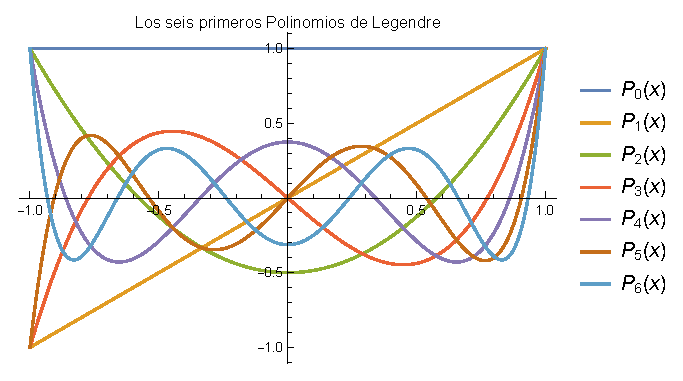
\includegraphics[scale=1.3]{Imagenes/Plot_Lagrange_0-6.eps}
    \caption{Gráfica de los primeros seis polinomios de Lagrange.}
    \label{fig:polinomios_Lagrange_01}
\end{figure}

A pesar de que si $\ell$ es un entero par o impar, respectivamente para $y_{1}(x)$ - ec. (\ref{eq:ecuacion_18_03}) - o $y_{2}(x)$ - ec. (\ref{eq:ecuacion_18_04}), se termina dando un múltiplo del correspondiente polinomio de Legendre $P_{\ell}(x)$, la otra serie en cada caso no termina y por tanto converge sólo para $\abs{x} < 1$.
\par
Dependiendo de si $\ell$ es par o impar, se definen las \emph{funciones de Legendre de segunda clase} como $Q_{\ell}(x) =  \alpha_{\ell} \, y_{2}(x)$ o $Q_{\ell}(x) =  \beta_{\ell} \, y_{1}(x)$, respectivamente, donde las constantes $\alpha_{\ell}$ y $\beta_{\ell}$ toman los valores
\begin{align}
\alpha_{\ell} &= \dfrac{(-1)^{\ell/2} \; 2^{\ell} \; [(\ell / 2)!]^{2}}{\ell!} \hspace{3.5cm} \mbox{ para $\ell$ par} \label{eq:ecuacion_18_05}\\[1em]
\beta_{\ell} &= \dfrac{(-1)^{(\ell + 1)/2} \; 2^{\ell - 1} \; \lbrace \left[ (\ell - 1) /2 \right] ! \rbrace^{2}}{\ell!} \hspace{1cm} \mbox{ para $\ell$ impar} \label{eq:ecuacion_18_06}
\end{align}

La normalización de los factores se elige de tal manera que $Q_{\ell}(x)$ obedece la misma relación de recurrencia de $P_{\ell}(x)$.
\par
La solución general para la ecuación de Legendre para enteros $\ell$ es por tanto
\begin{align}
y(x) = c_{1} \, P_{\ell}(x) + c_{2} \, Q_{\ell} (x) 
\label{eq:ecuacion_18_07}
\end{align}

Donde $P_{\ell}(x)$ es un polinomio de orden $\ell$, que converge para cualquier $x$, y $Q_{\ell}(x)$ es una serie infinita que converge sólo si $\abs{x} < 1$.
\par
Usando el método del Wronskiano, podemos obtener una forma cerrada para $Q_{\ell}(x)$:
\par
Una segunda solución para la ecuación de Legendre -ec. \ref{eq:ecuacion_18_01}), con $\ell = 0$ es
\begin{align}
\begin{aligned}[b]
y_{2}(x) &= P_{0}(x) \scaleint{6ex}_{\bs }^{x} \dfrac{1}{[P_{0}(u)]^{2}} \, \exp \left( \int^{u} \dfrac{2 \, v}{1 - v^{2}} \dd{v} \right) \dd{u} \\[0.5em]
&= \scaleint{6ex}_{\bs }^{x} \exp [ - \ln (1 - u^{2}) ] \dd{u} \\[0.5em]
&= \scaleint{6ex}_{\bs }^{x} 1\dfrac{\dd{u}}{(1 - u^{2})} = \dfrac{1}{2} \, \ln \left( \dfrac{1 + x}{1 - x} \right)
\end{aligned}
\label{eq:ecuacion_18_08}
\end{align}

En la segunda línea hemos utilizado el hecho de que $P_{0}(x)=1$.
\par
Lo que queda es ajustar la normalización de esta solución para que se corresponda con la ecuación (\ref{eq:ecuacion_18_05}). Expandiendo el logaritmo en la ec. (\ref{eq:ecuacion_18_08}) como una serie de Maclaurin, obtenemos
\begin{align*}
y_{2}(x) = x + \dfrac{x^{3}}{3} + \dfrac{x^{5}}{5} + \cdots \end{align*}

\begin{figure}[H]
    \centering
    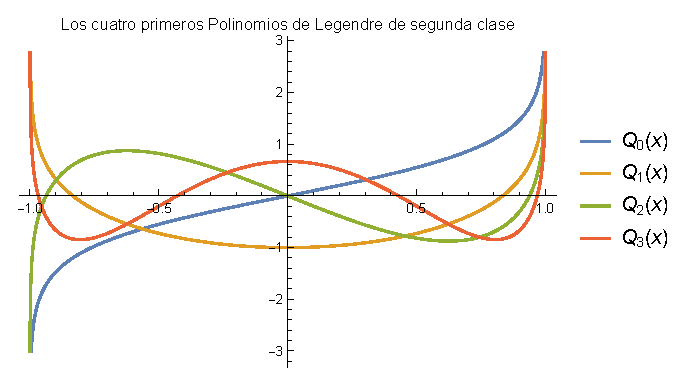
\includegraphics[scale=1.3]{Imagenes/Plot_LagrangeSC_0-4.eps}
    \caption{Gráfica de los cuatro polinomios de Lagrange de segunda clase.}
    \label{fig:polinomios_Lagrange_02}
\end{figure}

Comparando esto con la expresión para $Q_{0}(x)$, usando la ec. (\ref{eq:ecuacion_18_04}) con $\ell = 0$ y normalizando -ec. (\ref{eq:ecuacion_18_05})-, encontramos que $y_{2}$ está correctamente normalizada, así
\begin{align*}
Q_{0} (x) = \dfrac{1}{2} \, \ln \left( \dfrac{1 + x}{1 - x} \right)
\end{align*}

Usando el mismo método para $\ell = 1$, tenemos que
\begin{align*}
Q_{1} (x) =  \frac{1}{2} \, x \,  \ln \left( \dfrac{1 + x}{1 - x} \right) - 1
\end{align*}

Se pueden encontrar formas cerradas para $Q_{\ell}(x)$ de mayor orden, usando la relación de recurrencia.

\subsection{Propiedades de los Polinomios de Legendre.}

Como se mencionó anteriormente, cuando encontramos problemas físicos en donde la variable $x$ en la ecuación de Legendre es el coseno del ángulo polar $\theta$ en coordenadas esféricas, y entonces requiere la solución $y(x)$ que sea regular en $x = \pm 1$, que corresponde a $\theta = 0$ o $\theta = \pi$. Para que esto ocurra, requerimos que la ecuación tenga una solución polinomial, así el valor de $\ell$ debe ser un entero.
\par
Por otra parte, también requerimos que el coeficiente $c_{2}$ de la función $Q_{\ell}(x)$ en la ecuación (\ref{eq:ecuacion_18_07}) sea nulo, ya que $Q_{\ell}(x)$ es singular en $x = \pm 1$, como resultado de que la solución general es un múltiplo del polinomio de Legendre $P_{\ell}(x)$.

\subsection{Fórmula de Rodrigues.}

Como una ayuda para definir nuevas propiedades de los polinomios de Legendre, presentamos la \emph{fórmula de Rodrigues} para el $P_{\ell} (x)$:
\begin{align}
P_{\ell} (x) = \dfrac{1}{2^{\ell} \; \ell !} \dv[\ell]{x} \, (x^{2} - 1)^{\ell}
\label{eq:ecuacion_18_09}
\end{align}

\subsection{Ortogonalidad.}

Reconocemos que la ecuación de Legendre es de la forma Sturm-Liouville con $p = 1 - x^{2}$, $q = 0$, $\lambda = \ell (\ell + 1)$ y $\omega = 1$, y que su intervalo natural es $[-1, 1]$. Ya que los polinomios de Legendre $P_{\ell} (x)$ son regulares en los puntos extremos $x = \pm 1$, deben ser mutuamente ortogonales en este intervalo, es decir:
\begin{align}
\int_{-1}^{1} P_{\ell}(x) P_{k}(x) \dd{x} = 0 \hspace{1cm} \mbox{ si $\ell \neq k$}
\label{eq:ecuacion_18_12}
\end{align}

Como ya se comentó previamente, la ortogonalidad mutua (y completes) de $P_{\ell} (x)$ significa que cualquier función razonable $f(x)$ (es decir, una que satisfaga las condiciones de Dirichlet) puede expresarse en el intervalo de $\abs{x} < 1$ como una suma infinita de polinomios de Legendre:
\begin{align}
f(x) = \sum_{\ell = 0}^{\infty} a_{\ell} \, P_{\ell} (x)
\label{eq:ecuacion_013}
\end{align}

donde los coeficientes $a_{\ell}$ están dados por:
\begin{align}
a_{\ell} = \dfrac{2 \ell + 1}{2} \int_{-1}^{1} f(x) \, P_{\ell} (x) \dd{x}
\label{eq:ecuacion_18_14}
\end{align}

\subsection{Función generatriz.}

Una manera útil para manipular y estudiar secuencias de funciones o cantidades etiquetadas por una variable entera (en el caso de los polinomios de Legendre $P_{\ell} (x)$ están etiquetados por $\ell$), es mediante una función generatriz. 
\par
La función generatriz tiene quizás su mayor utilidad en el ámbito de la teoría de la probabilidad, sin embargo, también es de gran conveniencia en nuestro estudio.
\par
La función generatriz para decirlo, es una serie de funciones $f_{n} (x)$ para $n = 0, 1, 2,\ldots$ es una función $G (x, h)$ que contiene tanto a $x$, como una variable ficticia $h$, de tal manera que
\begin{align*}
G(x,h) = \sum_{n=0}^{\infty} f_{n} (x) \, h^{n}
\end{align*}

es decir, $f_{n}(x)$ es el coeficiente de $h^{n}$ en la expansión de $G$ en potencias de $h$. La utilidad de esta manera de trabajar la función, está en el hecho de que a veces es posible encontrar una forma cerrada para $G(x, h)$.
\par
En el caso de los polinomios de Legendre, usemos las funciones $P_{n}(x)$ definidas por:
\begin{align}
G(x ,h) = (1 - 2 \, x \, h + h^{2})^{-1/2} =  \sum_{n=0}^{\infty} P_{n}(x) \, h^{n}
\label{eq:ecuacion_18_15}
\end{align}

Como veremos las funciones así definidas son idénticas a los polinomios de Legendre y la función $(1 - 2 \, x \, h + h^{2})^{-1/2}$ es de hecho la función generatriz para ellos. En el proceso también vamos a deducir varias relaciones útiles entre los diferentes polinomios y sus derivadas.
\par
Hacemos la anotación de que $\dv*{P_{n}(x)}{x}$ es $\ptilde{P}_{n}$, derivamos la ecuación (\ref{eq:ecuacion_18_15}) con respecto a $x$ y obtenemos:
\begin{align}
h (1 - 2 \, x \, h + h^{2})^{-3/2} = \sum \ptilde{P}_{n} \; h^{n}
\label{eq:ecuacion_18_16}
\end{align}

También derivamos la ecuación (\ref{eq:ecuacion_18_15}) con respecto a $h$ por lo que:
\begin{align}
(x - h) (1 - 2 \, x \, h + h^{2})^{-3/2} = \sum n \; P_{n} \; h^{n-1}
\label{eq:ecuacion_18_17}
\end{align}

La ecuación (\ref{eq:ecuacion_18_16}) puede reescribirse usando la ecuación (\ref{eq:ecuacion_18_15}) como:
\begin{align*}
h \, \sum P_{n} \; h^{n} =  (1 - 2 \, x \, h + h^{2}) \sum \ptilde{P}_{n} \, h^{n}
\end{align*}

igualando los coeficientes de $h^{n+1}$, obtenemos la relación de recurrencia:
\begin{align}
P_{n} = \ptilde{P}_{n+1} - 2 \, x \; \ptilde{P}_{n} + \ptilde{P}_{n-1}
\label{eq:ecuacion_18_18}
\end{align}

Las ecuaciones (\ref{eq:ecuacion_18_16}) y (\ref{eq:ecuacion_18_17}) pueden combinarse como:
\begin{align*}
(x - h) \sum \ptilde{P}_{n} \; h^{n} = h \, \sum n \; P_{n} \; h^{n-1}
\end{align*}

donde el coeficiente de $h^{n}$ nos proporciona otra relación de recurrencia:
\begin{align}
x \, \ptilde{P}_{n} - \ptilde{P}_{n-1} =  n \; P_{n}
\label{eq:ecuacion_18_19}
\end{align}

eliminando $\ptilde{P}_{n-1}$ entre las ecuaciones (\ref{eq:ecuacion_18_18}) y (\ref{eq:ecuacion_18_19}), el resultado que se obtiene es:
\begin{align}
(n + 1) \, P_{n} = \ptilde{P}_{n+1} - x \; \ptilde{P}_{n}
\label{eq:ecuacion_18_20}
\end{align}

Si tomamos el resultado de la ecuación (\ref{eq:ecuacion_18_20}) reemplazando $n$ por $n-1$ y sumamos $x$ veces, obtenemos
\begin{align}
(1 - x^{2}) \, \ptilde{P}_{n} = n \; (P_{n-1} - x \, P_{n})
\label{eq:ecuacion_18_21}
\end{align}

Finalmente, derivamos ambos lados con respecto a $x$ y usamos el resultado de la ecuación (\ref{eq:ecuacion_18_19}) para tener
\begin{align*}
(1 - x^{2}) \stilde{P}_{n} - 2 \, x \, \ptilde{P}_{n} &= n \, \bigg[ (\ptilde{P}_{n-1} - x \, \ptilde{P}_{n}) - P_{n} \bigg] = \\[0.5em]
&= n \, (-n \, P_{n} - P_{n}) = \\[0.5em]
&= -n \, (n + 1) \, P_{n}
\end{align*}

por lo que los $P_{n}$ definidos en la ecuación (\ref{eq:ecuacion_18_15}), satisfacen la ecuación de Legendre.
\par
El ejemplo anterior muestra que las funciones $P_{n} (x)$ definida por la ecuación (\ref{eq:ecuacion_18_15}) satisfacen la ecuación de Legendre con $\ell = n$ (un entero) y también de (\ref{eq:ecuacion_18_15}), estas funciones son regulares en $x = \pm 1$. Por lo tanto $P_{n}$ debe ser un múltiplo del n-ésimo polinomio de Legendre. Por lo tanto, sólo queda verificar la normalización. Esto se hace fácilmente en $x = 1$, cuando $G$ se convierte en:
\begin{align*}
G(1, h) = [(1 - h)^{2}]^{-1/2} =  1 + h + h^{2} + \cdots
\end{align*}

y podemos ver que todo $P_{n}$ así definido, se tiene $P_{n} (1) = 1$ como se requiere, por tanto son idénticos a los polinomios de Legendre.
\par
Un uso particular de la función generatriz (\ref{eq:ecuacion_18_15}) es la representación del inverso de la distancia entre dos puntos en el espacio tridimensional en términos de polinomios de Legendre. Si dos puntos $\vb{r}$ y $\ptilde{\vb{r}}$ se encuentran a distancias $r$ y $\ptilde{r}$, respectivamente, desde el origen, con $\ptilde{r} < r$, se tiene que:
\begin{align}
\begin{aligned}[b]
\dfrac{1}{\abs{\vb{r} - \ptilde{\vb{r}}}} &= \dfrac{1}{(r^{2} + r^{\prime \: 2} - 2 \, r \, \ptilde{r} \, \cos \theta)^{1/2}} \\[0.5em]
&= \dfrac{1}{r \, [ 1 -2 (\ptilde{r}/r) \, \cos \theta + (\ptilde{r}/r)^{2}]^{1/2}} \\[0.5em]
&= \dfrac{1}{r} \sum_{\ell = 0}^{\infty} \left( \dfrac{\ptilde{r}}{r} \right)^{\ell} \, P_{\ell} (\cos \theta)
\end{aligned}
\label{eq:ecuacion_18_22}
\end{align}

donde $\theta$ es el ángulo entre los dos vectores de posición $\vb{r}$ y $\ptilde{\vb{r}}$. Si $\ptilde{r} > r$, entonces $r$ y $\ptilde{r}$ deben de intercambiarse en la ecuación (\ref{eq:ecuacion_18_22}) o de lo contrario, la serie no converge.
\par
Este resultado puede ser utilizado por ejemplo, para escribir el potencial electrostático en un punto $\vb{r}$ debido a una carga $q$ en el punto $\ptilde{\vb{r}}$. Entonces, en el caso $\ptilde{r} < r$, se tiene que:
\begin{align*}
V(\vb{r}) = \dfrac{q}{4 \, \pi \, \varepsilon_{0} \, r} \sum_{\ell=0}^{\infty} \left( \dfrac{\ptilde{r}}{r} \right)^{\ell} \, P_{\ell} (\cos \theta)
\end{align*}

Vemos el caso especial cuando la carga está en el origen, y $\ptilde{r} = 0$, entonces el término $\ell =0$ en la serie es no nulo, y la expresión se reduce a la forma ya conocida 
\begin{align*}
V(\vb{r}) = \dfrac{q}{4 \, \pi \, \varepsilon_{0} \, r}
\end{align*}

\subsection{Relaciones de recurrencia.}

En nuestro análisis previo de la función generatriz, derivamos varias relaciones de recurrencia útiles que satisfacen los polinomios de Legendre $P_{n} (x)$. En particular, a partir de la ecuación (\ref{eq:ecuacion_18_18}), tenemos la cuarta relación de recurrencia:
\begin{align*}
\ptilde{P}_{n+1} + \ptilde{P}_{n-1} =  P_{n} + 2 \; x \; \ptilde{P}_{n}
\end{align*}

De las ecuaciones (\ref{eq:ecuacion_18_19}) a (\ref{eq:ecuacion_18_21}) tenemos las siguientes relaciones de recurrencia con tres términos:
\begin{align*}
\ptilde{P}_{n+1} &= (n+1) \; P_{n} + x \; \ptilde{P}_{n} \\[0.5em]
\ptilde{P}_{n-1} &= -n \; P_{n} + x \; \ptilde{P}_{n} \\[0.5em]
(1 - x^{2}) \, \ptilde{P}_{n+1} &= n \; (P_{n-1} - x \; P_{n}) \\[0.5em]
(2 \, n + 1) \, P_{n} &= \ptilde{P}_{n+1} - \ptilde{P}_{n-1}
\end{align*}

\subsection{Ejemplo.}
\textbf{Ejemplo 1.} Queremos encontrar la expansión de Legendre de una función $f(x)$ definida por
\begin{align*}
f(x) = \begin{cases}
V_{0} & \mbox{ si } 0 < x \leq 1 \\[0.5em]
- V_{0} & \mbox{ si } -1 \leq x < 0
\end{cases}
\end{align*}

Utilizamos la ecuación (\ref{eq:ecuacion_18_14}) para determinar los coeficientes:
\begin{align*}
a_{\ell} &= \dfrac{2 \, \ell + 1}{2} \int_{-1}^{1} f(x) \, P_{\ell} (x) \dd{x} \\[0.5em]
&= \dfrac{2 \, \ell + 1}{2} \int_{-1}^{0} \underbrace{f(x)}_{=-V_0}  P_{\ell} (x) \dd{x} + \dfrac{2 \, \ell + 1}{2} \int_{0}^{1} \underbrace{f(x)}_{=+V_0} \, P_{\ell} (x) \dd{x} \\[0.5em]
&= \dfrac{2 \, \ell + 1}{2} \, V_{0} \left[ - \int_{-1}^{0} P_{\ell} (x) \dd{x} + \int_{0}^{1} P_{\ell} (x) \dd{x} \right]
\end{align*}

En la primera integral de la última línea, hacemos el cambio de variable $x = -y$, por lo que:
\begin{align*}
\int_{-1}^{0} P_{\ell} (x) \dd{x} = \int_{+1}^{0} P_{\ell} (-y) (-\dd{y}) = \int_{0}^{1} P_{\ell} (-y) \dd{y} = (-1)^{\ell} \, P_{\ell} (x) \dd{x}
\end{align*}

donde ocupamos una la propiedad de paridad de los polinomios de Legendre:
\begin{align*}
P_{\ell} (-u) = (-1)^{\ell} \, P_{\ell} (u)
\end{align*}

Sustituimos en la expresión para los coeficientes:
\begin{align*}
a_{\ell} &= \dfrac{2 \, \ell + 1}{2} \, V_{0} \,  [1 - (-1)^{\ell} \int_{0}^{1} P_{\ell} (x) \dd{x} \\[0.5em]
&= \dfrac{2 \, \ell + 1}{2} \, V_{0} \begin{cases}
0 & \mbox{ si } \ell \mbox{ es par} \\[0.5em]
2 \, \displaystyle \int_{0}^{1} P_{2k+1} (x) \dd{x} & \mbox{ si } \ell = 2 k + 1 
\end{cases}
\end{align*}

donde para $\ell$ impar se definió como $\ell = 2 \, k + 1$ con $k = 0, 1, 2, \ldots$.
\par

Queda por evaluar la integral del polinomio de Legendre de orden impar en el intervalo $(0, 1)$. Para ello, utilizamos la fórmula de Rodrigues:
\begin{align*}
\int_{0}^{1} P_{2k+1} (x) \dd{x} &= \dfrac{1}{2^{2k+1} \; (2 \, k +1)!} \int_{0}^{1} \dv[2k+1]{x} \left[ (x^{2} {-} 1)^{2k+1} \right] \dd{x} = \\[0.5em]
&= \dfrac{1}{2^{2k+1} \; (2 \, k +1)!} \; \dv[2k]{x} \left[ (x^{2} {-} 1)^{2k+1} \right] \eval_{0}^{1} = \\[0.5em]
&= \dfrac{1}{2^{2k+1} \; (2 \, k +1)!} \; \bigg[ \dv[2k]{x} \left[ (x^{2} {-} 1)^{2k+1} \right] \eval_{x=1} + \\[0.5em]
&- \dv[2k]{x} \left[ (x^{2} {-} 1)^{2k+1} \right] \eval_{x=0} \bigg]
\end{align*}

El primer término resulta ser cero, porque no hay un número suficiente de diferenciaciones para deshacerse de todos los factores de $(x^{2} - 1)$. Para el segundo término, observamos que $(x^{2} - 1)^{2k + 1}$ es un polinomio en $x$ cuyos derivadas de varios órdenes, serán potencias de $x$. Estas potencias devolverán cero en $x = 0$, excepto para el término constante (de potencia cero). Por lo tanto, vamos a utilizar la expansión binomial para $(x^{2} - 1)^{2k + 1}$, que es igual a $-(1 {-} x^{2})^{2k + 1}$:
\begin{align*}
\dv[2k]{x} \left[ (x^{2} {-} 1)^{2k+1} \right] \eval_{x=0} &= - \dv[2k]{x} \left[ \nsum_{j=0}^{2k+1} \dfrac{(2k+1)!}{j! \; (2k + 1 - j)!} \, (-x^{2})^{j} \right] \eval_{x=0} = \\[0.5em]
&= - \nsum_{j=0}^{2k+1} \dfrac{(2k+1)!}{j! \; (2k + 1 - j)!} (-1)^{j} \, \dv[2k]{x} \left( x^{2j} \right) \eval_{x=0}
\end{align*}

de donde se obtiene un término constante cuando $k = j$, todos los demás términos de la suma se anulan ya sea por tener  demasiadas diferenciaciones (cuando $j < k$, terminamos derivando constantes), o por tener muy pocas diferenciaciones (cuando $j > k$, una potencia de $x$ permanece y se evalúa como cero en $x = 0$). Por tanto:
\begin{align*}
\dv[2k]{x} \left[ (x^{2} {-} 1)^{2k+1} \right] \eval_{x=0} &= - \dfrac{(2k+1)!}{k! \; (2k + 1)!} (-1)^{k} \, \dv[2k]{x} \left( x^{2k} \right) \eval_{x=0} \\[0.5em]
&= \dfrac{(2k+1)!}{k! \; (2k + 1)!} (-1)^{k+1} \; (2k)!
\end{align*}

Entonces el coeficiente $a_{2k+1}$ se escribe como
\begin{align*}
a_{2k+1} = 2 \, \dfrac{2 \, (2 \, k + 1) + 1}{2} \; V_{0} \int_{0}^{1} P_{2k+1} (x) \dd{x} = \dfrac{(-1)^{k} \, (4 \, k + 3)(2 \, k!)}{2^{2k+1} \; k! \; (k+1)!} \, V_{0}
\end{align*}

con $a_{\ell} = 0$ para $\ell$ par. La expansión en series de la función $f(x)$ se escribe como:
\begin{align*}
f(x) = \begin{cases}
V_{0} & \mbox{ si } 0 < x \leq 1 \\[0.5em]
-V_{0} & \mbox{ si } -1 \leq x < 0
\end{cases}
= V_{0} \nsum_{k=0}^{\infty} \dfrac{(-1)^{k}(4 \, k + 3)(2 \, k!)}{2^{2k+1} \; k! \; (k+1)!} P_{2k+1} (x)
\end{align*}

Expresando los primeros términos :
\begin{align*}
f(x) = V_{0} \left[ \dfrac{3}{2} \, P_{1}(x) - \dfrac{7}{8} \, P_{3}(x) + \dfrac{11}{16} \, P_{5}(x) - \cdots \right]
\end{align*}


\section{Funciones asociadas de Legendre.}

La ecuación diferencial asociada de Legendre tiene la forma:
\begin{align}
(1 - x^{2}) \, \stilde{y} - 2 \, x \, \ptilde{y} + \left[ \ell (\ell + 1) - \dfrac{m^{2}}{1 - x^{2}} \right] \, y = 0
\label{eq:ecuacion_18_28}
\end{align}

que tiene tres puntos singulares en $x = -1, 1, \infty$, se reduce a la ecuación de Legendre cuando $m=0$, vista en el numeral anterior.
\par
Se presenta en problemas de la física que involucran el operador $\nabla^{2}$, cuando se expresa en coordenadas polares. En esos casos, $- \ell \leq m \leq \ell$ y $m$ está restringida a valores enteros.
\par
Como en el caso de la ecuación de Legendre, la variable $x$ es el coseno del ángulo polar en coordenadas esféricas, por tanto $-1 \leq x \leq 1$. Cualquier solución de la ecuación diferencial \ref{eq:ecuacion_18_28}) es llamada la \emph{función asociada de Legendre}.
\par
El punto $x = 0$ es un punto ordinario, y del cual se pueden obtener soluciones en series de la forma:
\begin{align*}
y = \sum_{n=0} a_{n} \, x^{n}
\end{align*}

de la misma manera que se hizo para la ecuación de Legendre. En este caso, debemos de notar que si $u(x)$ es solución de la ecuación de Legendre, entonces:
\begin{align}
y(x) = (1 -x^{2})^{\abs{m}/2} \dv[\abs{m}]{u}{x}
\label{eq:ecuacion_18_29}
\end{align}

es solución a la ecuación asociada (\ref{eq:ecuacion_18_28}).
\par
Veamos que si $u(x)$ es solución de la ecuación de Legendre, entonces $y(x)$ dada por la ec. (\ref{eq:ecuacion_18_29}) es una solución a la ecuación asociada de Legendre:
\par
Por simplicidad, consideremos que $m$ no es negativo, la ecuación de Legendre para $u$ es:
\begin{align*}
(1 - x^{2}) \, \stilde{y} - 2 \, x \, \ptilde{y} + \left[ \ell (\ell + 1) \right] \, y = 0
\end{align*}

al diferenciar $m$ veces esta ecuación mediante el teorema de Leibinz, obtenemos:
\begin{align}
(1 - x^{2}) \, \stilde{v} - 2 \, x \, (m + 1) \, \ptilde{v} + \left[ \ell - m) (\ell + m + 1) \right] \, v = 0
\label{eq:ecuacion_18_30}
\end{align}

donde $v(x) = \dv*[m]{u}{x}$.
\par
Definiendo:
\begin{align*}
y(x) = (1 - x^{2}) ^{m/2} \, v(x)
\end{align*}

Las derivadas de $\ptilde{v}$ y $\stilde{v}$ se pueden escribir como:
\begin{align*}
\ptilde{v} &= (1 - x^{2})^{-m/2} \, \left( \ptilde{y} + \dfrac{m \, x}{1 -x^{2}} \, y \right) \\[1em]
\stilde{v} &= (1 - x^{2})^{-m/2} \, \left[ \stilde{y} + \dfrac{2 \, m \, x}{1 -x^{2}} \, \ptilde{y} + \dfrac{m \, x}{1 -x^{2}} \, y + \dfrac{m(m + 2) \, x^{2}}{(1 -x^{2})^{2}} \, y \right]
\end{align*}

Sustituyendo las expresiones en la ec. (\ref{eq:ecuacion_18_30}), para luego simplificar llegamos a:
\begin{align*}
(1 - x^{2}) \, \stilde{y} - 2 \, x \, \ptilde{y} + \left[ \ell (\ell + 1) - \dfrac{m^{2}}{1 - x^{2}} \right] \, y = 0
\end{align*}

lo que demuestra que $y$ es solución a la ecuación asociada de Legendre (\ref{eq:ecuacion_18_28}). En caso de que $m$ sea negativo, el valor de $m^{2}$ no se modifica, por lo que una solución para $m$ positivo, es también una solución para el correspondiente valor de $m$ negativo.
\par
De las dos soluciones en serie linealmente independientes de la ecuación de Legendre dada por:
\begin{align*}
y_{1}(x) &= 1 - \ell (\ell + 1) \dfrac{x^{2}}{2!} + (\ell - 2)\; \ell \; (\ell + 1)\;(\ell + 3) \dfrac{x^{4}}{4!} - \ldots \\[1em]
y_{2}(x) &= x - (\ell - 1)(\ell + 2) \dfrac{x^{3}}{3!} + (\ell - 3) (\ell - 1)(\ell + 2)(\ell + 4) \dfrac{x^{5}}{5!} - \ldots
\end{align*}

que ahora denotamos por $u_{1} (x)$ y $u_{2}(x)$, podemos obtener dos soluciones en serie linealmente independientes, $y_{1} (x)$ y $y_{2} (x)$, a la ecuación asociada de Legendre mediante el uso de (\ref{eq:ecuacion_18_29}). A partir de la discusión general de la convergencia de la serie de potencias, vemos que ambas $y_{1} (x)$ y $y_{2} (x)$ también convergen para $\abs{x} < 1$. Por lo tanto la solución general de la ecuación(\ref{eq:ecuacion_18_28}) en este rango está dado por:
\begin{align*}
y(x) = c_{1} \, y_{1} (x) + c_{2} \, y_{2} (x)
\end{align*}

\subsection{Funciones asociadas de Legendre para enteros \texorpdfstring{$\ell$}{l}.}

Si $\ell$ y $m$ son ambos enteros, como en el caso de varios problemas de la física, entonces la solución general de la ecuación (\ref{eq:ecuacion_18_28}) se expresa por:
\begin{align}
y(x) = c_{1} \, P_{\ell}^{m} (x) + c_{2} \, Q_{\ell}^{m} (x)
\label{eq:ecuacion_18_31}
\end{align}

donde $P_{\ell}^{m} (x)$ y $Q_{\ell}^{m} (x)$ son las funciones asociadas de Legendre de primera y segunda clase, respectivamente. Para valores no negativos de $m$, esas funciones están relacionadas a las funciones de Legendre para enteros $\ell$ mediante:
\begin{align}
\begin{aligned}
P_{\ell}^{m} (x) &= (1 - x^{2})^{m/2} \dv[m]{P_{\ell}}{x}, \\[1em]
Q_{\ell}^{m} (x) &= (1 - x^{2})^{m/2} \dv[m]{Q_{\ell}}{x}
\end{aligned}
\label{eq:ecuacion_18_32}
\end{align}

Vemos inmediatamente que, en caso necesario, las funciones asociadas de Legendre se reducen a las funciones ordinarias de Legendre cuando $m = 0$. 
\par
Dado que $m^{2}$ aparece en la ecuación asociada de Legendre -ec. (\ref{eq:ecuacion_18_28})-, las funciones asociadas de Legendre para los valores negativos $m$ debe ser proporcional a la función correspondiente para valores no negativos $m$. La constante de proporcionalidad es una cuestión de convención. Para el $P_{\ell}^{m} (x) $, es habitual considerar la definición (\ref{eq:ecuacion_18_32}) como válida también para los valores negativos $m$. Aunque la diferenciación de un número negativo no está definida, cuando $P_{\ell}(x)$ se expresa en términos de la fórmula de Rodrigues (de los polinomios de Legendre), este problema no se presenta para $\ell \leq m \leq \ell$. En este caso:
\begin{align}
P_{\ell}^{-m} (x) = (-1)^{m} \; \dfrac{(\ell - m)!}{(\ell + m)!} \, P_{\ell}^{m} (x)
\label{eq:ecuacion_18_33}
\end{align}

Ya que $P_{\ell}(x)$ es un polinomio de orden $\ell$, tenemos que $P_{\ell}^{m}(x)=0$ para $\abs{m} > \ell$. De esta definición, queda claro que $P_{\ell}^{m} (x)$ es también un polinomio de orden $\ell$ si $m$ es par, ya que contiene el factor $(1-x^{2})$ a una potencial fraccionaria si $m$ es impar. En cualquier caso $P_{\ell}^{m}(x)$ es regular en $x = \pm 1$.
\par
Los primeros polinomios asociados de Legendre de primera clase, se construyen fácilmente y están dadas por (se omiten los casos $m=0$):
\begin{align*}
P_{1}^{1} (x) &= (1 - x^{2})^{1/2} \\[0.5em]
P_{2}^{1} (x) &= 3 \, x \, (1 - x^{2})^{1/2} \\[0.5em]
P_{2}^{2} (x) &= 3 \, (1 - x^{2}) \\[0.5em]
P_{3}^{1} (x) &= \dfrac{3}{2}(5 \, x^{2} - 1)(1 - x^{2})^{1/2} \\[0.5em]
P_{3}^{2} (x) &= 15 \, x (1 - x^{2}) \\[0.5em]
P_{3}^{3} (x) &= 15 \, (1 - x^{2})^{3/2}
\end{align*}

\begin{figure}[H]
    \centering
    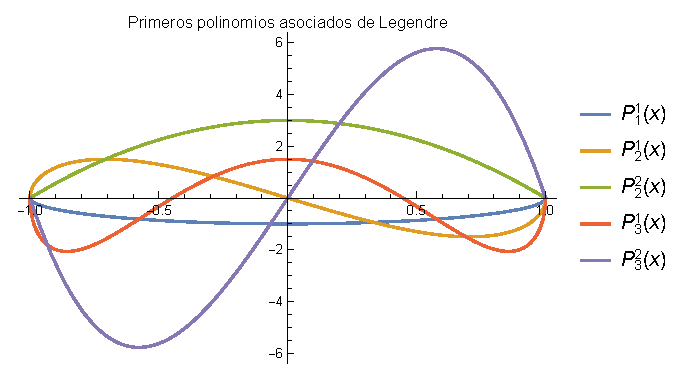
\includegraphics[scale=1.3]{Imagenes/Plot_Asociados_Lagrange.eps}
    \caption{Gráfica de los primeros polinomios asociados de Legendre, no se incluyen aquellos con $m = 0$.}
    \label{fig:figura_asociados_Legedre}
\end{figure}

Debemos de mencionar que las funciones asociadas de Legendre de segunda clase $Q_{\ell}^{m} (x)$ como las $Q_{\ell}(x)$ son singulares en $x = \pm 1$.

\subsection{Propiedades de las funciones asociadas de Legendre \texorpdfstring{$P_{\ell}^{m}$}{Plm}.}

Cuando encontramos en problemas físicos, la variable $x$ de la ecuación asociada de Legendre (como en la ecuación ordinaria Legendre) es generalmente el coseno del ángulo polar $\theta$ en coordenadas polares esféricas, y entonces queremos que la solución $y (x)$ sea regular en $x = \pm 1$ (correspondiente a $\theta = 0$ o $\theta = \pi$). Para que esto ocurra, se requiere que $\ell$ sea un número entero y que el coeficiente $c_{2}$ de la función $Q_{\ell}^{m} (x)$ en la ecuación (\ref{eq:ecuacion_18_31}) sea cero, dado que $Q_{\ell}^{m}(x)$ es singular en $x = \pm 1$, con el resultado de que la solución general son múltiplos de las funciones asociadas de Legendre de primera clase $P_{\ell}^{m}(x)$.

\subsection{Ortogonalidad mutua.}

Ya se mencionó anteriormente que la ecuación asociada de Legendre es del tipo Sturm-Liouville de la forma:
\begin{align*}
\ptilde{(p \, y)} + q \, y + \lambda \,  \omega \, y = 0
\end{align*}

con
\begin{align*}
p &= 1 - x^{2} \\[0.5em]
q &= - \dfrac{m^{2}}{(1 - x^{2})} \\[0.5em]
\lambda &= \ell (\ell + 1) \\[0.5em]
\omega &= 1
\end{align*}

siendo su intervalo natural en $[-1,1]$.
\par
Dado que las funciones asociadas de Legendre $P_{\ell}^{m} (x)$ son regulares en los extremos $x = \pm 1$, entonces deben de ser mutuamente ortogonales en este intervalo para un valor fijo de $m$, es decir:
\begin{align}
\int_{-1}^{1} P_{\ell}^{m} (x) \, P_{k}^{m} (x) \dd{x}  = 0, \hspace{1cm} \mbox{ si } \ell \neq	 k
\label{eq:ecuacion_18_36}
\end{align}

Nótese que el valor de $m$ debe de ser el mismo en ambas funciones asociadas de Legendre para que la expresión sea válida. La condición de normalización cuando $\ell = k$ se obtiene de la fórmula de Rodrigues:
\begin{align}
I_{\ell m} = \int_{-1}^{1} P_{\ell}^{m} (x) \, P_{\ell}^{m} (x) \dd{x} = \dfrac{2}{2 \, \ell + 1} \, \dfrac{(\ell + m)!}{( \ell - m)!}
\label{eq:ecuacion_18_37}
\end{align}

Las condiciones de ortogonalidad y normalización, ecuaciones (\ref{eq:ecuacion_18_36}) y (\ref{eq:ecuacion_18_37}), respectivamente, significan que los polinomios asociados de Legendre $P_{\ell}^{m}(x)$, con $m$ fija, puede utilizarse de manera similar a los polinomios de Legendre para expandir cualquier función $f(x)$ razonable en el intervalo $\abs{x} < 1$ en una serie de la forma:
\begin{align}
f(x) = \sum_{k=0}^{\infty} a_{m+k} \, P_{m+k}^{m} (x)
\label{eq:ecuacion_18_38}
\end{align}

donde los coeficientes están dados por:
\begin{align*}
a_{\ell} = \dfrac{2 \, \ell + 1}{2} \, \dfrac{(\ell - m)!}{(\ell + m)!} \int_{-1}^{1} f(x) \, P_{\ell}^{m} (x) \dd{x}
\end{align*}

\subsection{Función generatriz.}

La función generatriz para las funciones asociadas de Legendre, se obtienen de la combinación de su definición con la función generatriz de los polinomios de Legendre:
\begin{align}
G(x, h) = \dfrac{(2 \, m)(1 - x^{2})^{m/2}}{2^{m} \, m! \, (1 - 2 \, h \, x + h^{2})^{m+1/2}} = \sum_{n=0}^{\infty} P_{n+m}^{m} (x) \, h^{n}
\label{eq:ecuacion_18_40}
\end{align}

\subsection{Relaciones de recurrencia.}

Como era de esperar, las funciones asociadas de Legendre satisfacen ciertas relaciones de recurrencia. De hecho, la presencia de los dos índices $n$ y $m$ significa que se puede derivar una gama mucho más amplia de relaciones de recurrencia. Presentaremos sólo cuatro de las relaciones más útiles:
\begin{align*}
P_{n}^{m+1} &= \dfrac{2 \, m \, x}{(1 - x^{2})^{1/2}} P_{n}^{m} + [m (m - 1) - n (n + 1)] \, P_{n}^{m-1} \\[0.5em]
(2 \, n + 1) \, x \, P_{n}^{m} &= (n + m) \, P_{n-1}^{m} + (n - m + 1) \, P_{n+1}^{m} \\[0.5em]
(2 \, n + 1)(1 -  x^{2})^{1/2} P_{n}^{m} &= P_{n+1}^{m+1} - P_{n-1}^{m+1} \\[0.5em]
2 \, (1 - x^{2})^{1/2} \ptilde{(P_{n}^{m})} &= P_{n}^{m+1} - (n + m)(n - m + 1) \, P_{n}^{m-1}
\end{align*}

Las relaciones de recurrencia son válidas tanto para valores negativos como positivos de $m$.

\section{Armónicos esféricos.}

Las funciones asociadas de Legendre discutidas anteriormente se presentan más comúnmente la solución de la ecuación de Laplace $\laplacian =0$ en coordenadas polares esféricas. En particular, se encuentra que para las soluciones que son finitas en el eje polar, la parte angular de la solución viene dada por:
\begin{align*}
\Theta (\theta) \, \Phi (\phi) = P_{\ell}^{m} (\cos \theta) \, (C \,  \cos m \phi + D \, \sin m \phi)
\end{align*}

donde $\ell$ y $m$ son enteros con $- \ell \leq m \leq \ell$. Esta forma general es muy común para funciones particulares de $\theta$ y $\phi$, se les llama \emph{armónicos esféricos}, se definen por:
\begin{align}
Y_{\ell}^{m} (\theta, \phi) = (1-)^{m} \left[ \dfrac{2 \ell + 1}{4 \, \pi} \: \dfrac{(\ell + m)!}{(\ell - m)!} \right]^{1/2} \, P_{\ell}^{m} (\cos \theta) \exp(i \, m \, \phi)
\label{eq:ecuacion_18_45}
\end{align}

Usando la ecuación (\ref{eq:ecuacion_18_33}), encontramos que:
\begin{align*}
Y_{\ell}^{-m} (\theta, \phi) =  (-1)^{m} \left[ Y_{\ell}^{m} (\theta,\phi) \right]^{*}
\end{align*}

donde el asterisco indica el complejo conjugado. Los primeros armónicos esféricos $Y_{\ell}^{m}(\theta,\phi) \equiv Y_{\ell}^{m}$ son:
\begin{align*}
Y_{0}^{0} &= \sqrt{\dfrac{1}{4 \, \pi}} \\[0.5em]
Y_{1}^{0} &= \sqrt{\dfrac{3}{4 \, \pi}} \cos \theta \\[0.5em]
Y_{1}^{\pm 1} &= \mp \sqrt{\dfrac{3}{8 \, \pi}} \sin \theta \exp(\pm i \, \phi) \\[0.5em]
Y_{2}^{0} &= \sqrt{\dfrac{5}{16 \, \pi}} ( 3 \, \cos^{2} \theta - 1) \\[0.5em]
Y_{2}^{\pm 1} &= \mp \sqrt{\dfrac{15}{8 \, \pi}} \sin \theta \, \cos \theta \exp(\pm i \, \phi) \\[0.5em]
Y_{2}^{\pm 2} &= \sqrt{\dfrac{15}{32 \, \pi}} \sin^{2} \theta \exp(\pm 2 \, i \, \phi)
\end{align*}

Estas funciones se pueden visualizar haciendo una gráfica en coordenadas polares en tres dimensiones de:
\begin{align*}
\abs{Y_{\ell}^{m} (\theta, \phi)}^{2} \hspace{0.2cm} \mbox{ contra } \theta \mbox{ y } \phi
\end{align*}

La gráfica para $Y_{0}^{0} (\theta, \phi)$ se muestra en la figura (\ref{fig:armonico_esferico_00}), donde la magnitud al cuadrado del armónico esférico está representado por la distancia del origen a la superficie.
\begin{figure}[H]
    \centering
    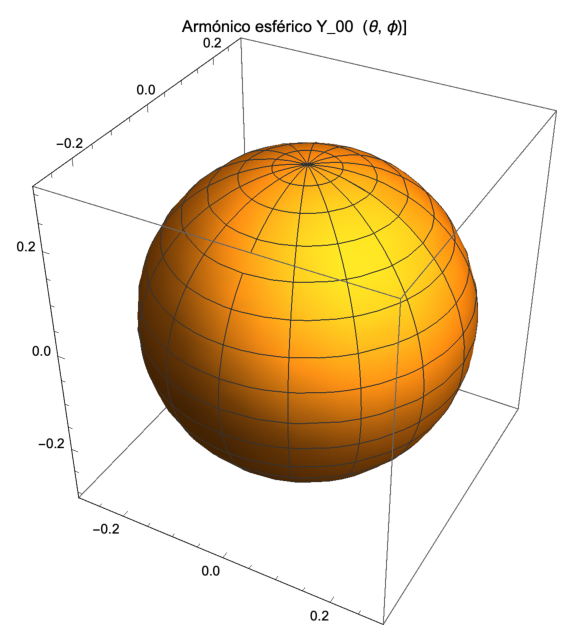
\includegraphics[scale=1]{Imagenes/Armonicos_Esfericos_00.eps}
    \label{fig:armonico_esferico_00}
\end{figure}

Las superficies similares se muestran para los armónicos esféricos $\ell = 1$ y $\ell = 2$; en éstas figuras, el eje $z$ es vertical, y las superficies son siempre simétricas sobre el eje, ya que $\abs{\exp(i \, m \, \phi)} = 1$. Por tanto, las gráficas para $\pm m$ son siempre las mismas, ya que:
\begin{align*}
\abs{Y_{\ell}^{m}} = \abs{Y_{\ell}^{-m}}
\end{align*}

\newpage
\begin{figure}[H]
    \centering
    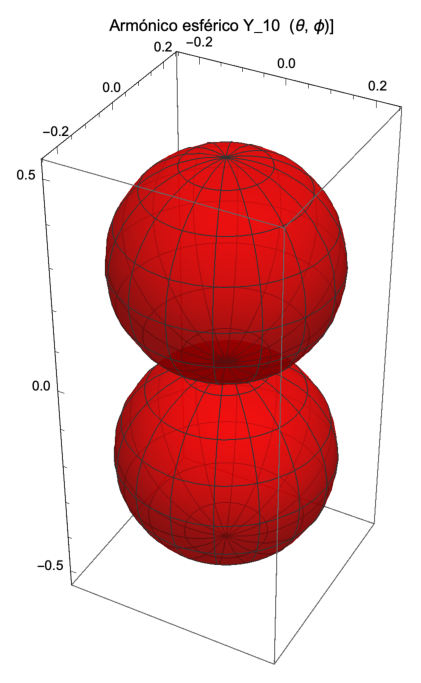
\includegraphics[scale=1]{Imagenes/Armonicos_Esfericos_10.eps}
    
    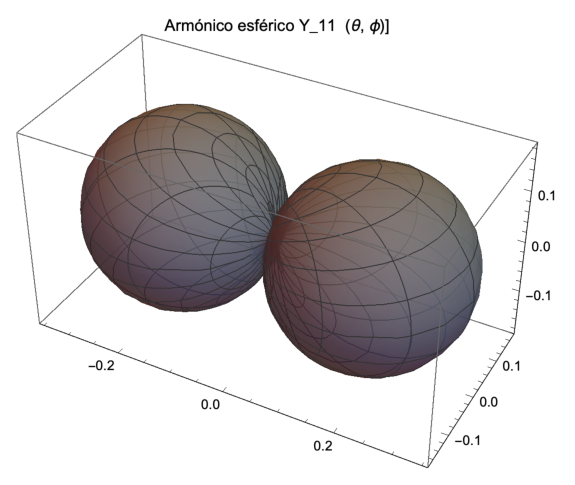
\includegraphics[scale=1]{Imagenes/Armonicos_Esfericos_11.eps}
\end{figure}
\newpage
\begin{figure}[H]
    \centering
    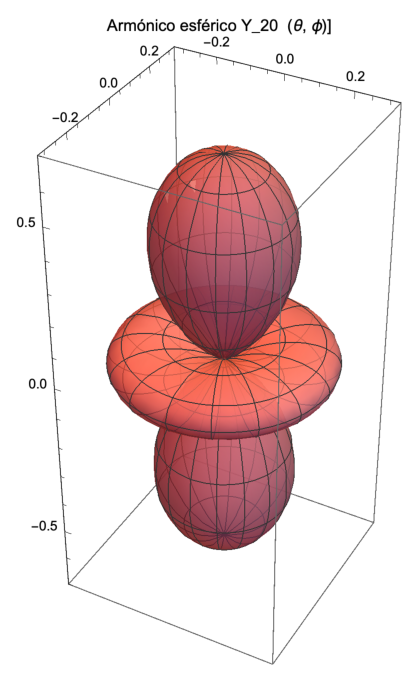
\includegraphics[scale=1]{Imagenes/Armonicos_Esfericos_20.eps}
 
    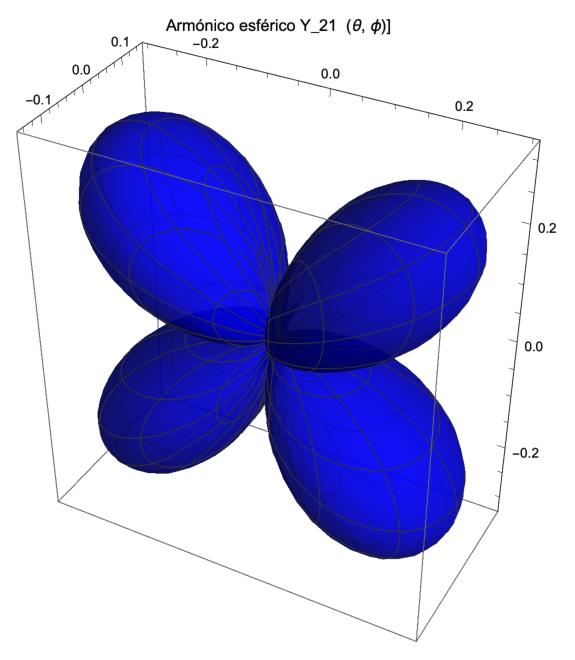
\includegraphics[scale=1]{Imagenes/Armonicos_Esfericos_21.eps}
\end{figure}
    
\subsection{Ortogonalidad mutua.}

Ya que contienen su parte $\theta$-dependiente de la solución $P_{\ell}^{m}$ a la ecuación asociada de Legendre, el $Y_{\ell}^{m}$ son mutuamente ortogonales cuando se integra de $-1$ a $+1$ sobre $\dd{cos \theta}$.
\par
Su ortogonalidad mutua respecto de $\phi \, (0 \leq \phi \leq 2 \pi)$ es aún más evidente. El factor numérico en la ecuación (\ref{eq:ecuacion_18_45}) es elegido para hacer el $Y_{\ell}^{m}$ un conjunto ortonormal, es decir:
\begin{align}
\int_{-1}^{1} \int_{0}^{2 \pi} [ Y_{\ell}^{m} (\theta, \phi) ]^{*} Y_{\ptilde{\ell}}^{\ptilde{m}} (\theta, \phi) \dd{\phi} \dd{(\cos \theta)} = \delta_{\ell \ptilde{\ell}} \,  \delta_{m \ptilde{m}}
\label{eq:ecuacion_18_46}
\end{align}

Adicionalmente, los armónicos esféricos forman un conjunto completo para cualquier función razonable de $\theta$ y $\phi$(como las que podemos encontrar en un problema físico), la función puede expandirse como una suma de tales funciones
\begin{align}
f(\theta, \phi) = \sum_{\ell=0}^{\infty} \sum_{-\ell}^{\ell} a_{\ell m} \, Y_{\ell}^{m} (\theta, \phi)
\label{eq:ecuacion_18_47}
\end{align}

las constantes $a_{\ell m}$ están dadas por:
\begin{align}
a_{\ell m} = \int_{-1}^{1} \int_{0}^{2 \pi} [ Y_{\ell}^{m} (\theta, \phi) ]^{*} f (\theta, \phi) \dd{\theta} \dd{(\cos \theta)}
\label{eq:ecuacion_048}
\end{align}

Esto es una analogía exacta con una serie de Fourier y es un ejemplo particular de la propiedad general de soluciones de Sturm-Liouville.

\subsection{Teorema del desarrollo.}

Parte de la importancia de los armónicos esféricos se encuentra en la propiedad de completes, una consecuencia de la forma de Sturm-Liouville de la ecuación de Laplace.
\par
Esta propiedad, en este caso, significa que cualquier función $f(\theta, \phi)$, con las suficientes propiedades de continuidad, evaluada sobre la superficie de una esfera se puede desarrollar en una serie convergente de manera uniforme en los armónicos esféricos, que se le conoce como \emph{Serie de Laplace}:
\begin{align}
f(\theta, \phi) = \sum_{m, \ell} a_{m \ell} \, Y_{\ell}^{m} (\theta, \phi)
\label{eq:ecuacion_12_151}
\end{align}

Si $f(\theta, \phi)$ es conocida, los coeficientes se pueden encontrar de inmediato mediante el uso de la integral de ortogonalidad:
\begin{align}
a_{m \ell} = \int f(\theta, \phi) \, (Y_{\ell}^{m})^{*} (\theta, \phi) \dd{\Omega}
\label{eq:ecuacion_10_237}
\end{align}

donde $\dd{\Omega}$ es el elemento de ángulo sólido de la esfera.
\par
Haciendo un cambio de variable, es posible demostrar que:
\begin{align}
\sum_{l \geq 0} \, \sum_{m=-\ell}^{\ell} Y_{\ell}^{m}) (\theta, \phi) \, (Y_{\ell}^{m})^{*} (\ptilde{\theta}, \ptilde{\phi}) = \delta(\phi - \ptilde{\phi}) \, \delta(\cos \theta  \cos \ptilde{\theta})
\label{eq:ecuacion_10_238}
\end{align}

A esta igualdad se le llama \emph{relación de completes}.

\subsection{Teorema de adición.}

Aparte de la condición ortonormalidad (\ref{eq:ecuacion_18_46}), la relación más importante que cumplen los $Y_{\ell}^{m}$ es el teorema de adición de armónicos esféricos:
\begin{align}
P_{\ell} (\cos \gamma) = \dfrac{4 \, \pi}{2 \, \ell + 1} \sum_{m = -\ell}^{\ell} Y_{\ell}^{m} (\theta, \phi) \, [ Y_{\ell}^{m} (\theta^{\prime}, \ptilde{\phi})]^{*}
\label{eq:ecuacion_18_49}
\end{align}

donde $(\theta, \phi)$ y $(\theta^{\prime}, \phi^{\prime})$ denotan dos direcciones diferentes a nuestro sistema de coordenadas esféricas polares y que están separadas por un ángulo $\gamma$. En general, la trigonometría esférica (o vectorial) demuestra que estos ángulos obedecen la identidad
\begin{align}
\cos \gamma = \cos \theta \, \cos \ptilde{\theta} + \sin \theta \, \sin \ptilde{\theta} \, \cos (\phi - \ptilde{\phi})
\label{eq:ecuacion_18_50}
\end{align}
El teorema de adición de los armónicos esféricos tiene bastantes aplicaciones, por ejemplo si $\theta = \ptilde{\theta}$ y $\phi = \ptilde{\phi}$, entonces la ec. (\ref{eq:ecuacion_18_49}) toma la forma
\begin{align}
\sum_{m = -\ell}^{\ell} \abs{Y_{\ell}^{m} (\theta, \phi)}^{2} = \dfrac{2 \, \ell + 1}{4 \, \pi}
\label{eq:ecuacion_10_262}
\end{align}
que se le llama \emph{regla de suma de los armónicos esféricos}.

%Referencia: Griffiths - 4.1.3 The radial equation

 \section{El átomo de hidrógeno - Parte radial.}

En la revisión de la parte angular de la función de onda $Y(\theta, \phi)$ es la misma para todo potencial esférico simétrico; la forma para el potencial en la parte angular $V(r)$, \emph{afecta solo la parte radial} de la función de onda $R(r)$, que queda determinada por la ec. (\ref{eq:ecuacion_04_16}):
\begin{align*}
\dfrac{1}{R} \, \dv{r} \left( r^{2} \, \dv{R}{r} \right) - \dfrac{2 \, m \, r^{2}}{\hbar^{2}} \bigg( V(r) - E \bigg) &= \ell (\ell + 1)
\end{align*}

esta ecuación se simplifica si hacemos el cambio de variable:
\begin{align}
u(r) = r \, R(r)
\label{eq:ecuacion_04_36}
\end{align}

por lo que:
\begin{align*}
R &= \dfrac{u}{r} \\[0.5em]
\dv{R}{u} &= \dfrac{ \big[ r \, \displaystyle \dv{u}{r} - u \big]}{r^{2}} \\[0.5em]
\dv{r} \, \bigg[ r^{2} \, \left( \dv{R}{r} \right) \bigg] &= r \, \dv[2]{u}{r}
\end{align*}

por tanto:
\begin{align}
- \dfrac{\hbar^{2}}{2 \, m} \, \dv[2]{u}{r} + \bigg[ V + \dfrac{\hbar^{2}}{2 \, m} \,\dfrac{\ell (\ell + 1)}{r^{2}} \bigg] \, u =  E \, u
\label{eq:ecuacion_04_37}
\end{align}

Esta ecuación es llamada \textbf{ecuación radial}, que es idéntica en forma a la ecuación de Schrödinger unidimensional, excepto por un potencial efectivo:
\begin{align*}
V_{\mbox{eff}} = V + \dfrac{\hbar^{2}}{2 \, m} \,\dfrac{\ell (\ell + 1)}{r^{2}}
\label{eq:ecuacion_04_38}
\end{align*}

que contiene un elemento adicional llamado \emph{término centrífugo}, que dirige a la partícula hacia afuera (lejos del origen), de la misma manera que ocurre en la fuerza centrífuga de la mecánica clásica.
\par
Para seguir avanzando en el estudio de la ecuación, se requiere conocer la manera del potencial.

\subsection{Potencial en el átomo de hidrógeno.}

El átomo de hidrógeno consta de un protón pesado, esencialmente inmóvil (de tal manera que podemos ponerlo en el origen) de carga $e$, junto con un electrón mucho más ligero (de carga $-e$) que se desplaza en círculo alrededor del protón, y se mantiene en órbita por la atracción mutua de cargas opuestas (ver Figura \ref{fig:figura_01}).
\begin{figure}[H]
    \centering
    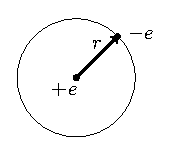
\includegraphics[scale=1.5]{Imagenes/atomohidrogeno.eps}
    \caption{El átomo de hidrógeno.}
    \label{fig:figura_01}
\end{figure}

A partir de la ley de Coulomb, la energía potencial (en unidades SI) es:
\begin{align}
V(r) = - \dfrac{e^{2}}{4 \, \pi \, \epsilon_{0}} \, \dfrac{1}{r}
\end{align}

y la ecuación radial (\ref{eq:ecuacion_04_37}) es:
\begin{align}
- \dfrac{\hbar^{2}}{2 \, m} \; \dv[2]{u}{r} + \left[ - \dfrac{e^{2}}{4 \, \pi \, \epsilon_{0}} \; \dfrac{1}{r} + \dfrac{\hbar^{2}}{2 \, m} \; \dfrac{\ell(\ell +1)}{r^{2}} \right] \, u =  E \, u
\label{eq:ecuacion_04_53}
\end{align}

Nuestro problema es resolver esta ecuación para $u(r)$ y determinar las energías permitidas $E$ de los electrones. 
\par
El potencial de Coulomb admite estados continuos (con $E > 0$), describiendo la dispersión  electrón - protón, así como estados ligados discretos, representando el átomo de hidrógeno, pero nos limitaremos nuestra atención a este último.

\subsection{La función radial de onda.}

Nuestra primera tarea es poner en orden la notación. Dejando:
\begin{align}
\kappa \equiv \dfrac{\sqrt{-2 \, m \, E}}{\hbar}
\label{eq:ecuacion_04_54}
\end{align}

(Para estados base, $E < 0$, por lo que $\kappa$ es real). Al dividir la ec. (\ref{eq:ecuacion_04_53}) por $E$, tenemos
\begin{align*}
\dfrac{1}{\kappa^{2}} \, \dv{2}{u}{r} = \left[1 - \dfrac{m \, e^{2}}{2 \, \pi \, \epsilon_{0} \,\hbar^{2} \kappa} \, \dfrac{1}{(\kappa \, r)} + \dfrac{\ell (\ell + 1)}{(\kappa \, r)^{2}} \right] \, u
\end{align*}

donde podemos hacer
\begin{align}
\rho \equiv \kappa \, r \hspace{1cm} \rho_{0} \equiv \dfrac{m \, e^{2}}{2 \, \pi \, \epsilon_{0} \, \hbar^{2} \, \kappa}
\label{eq:ecuacion_04_55}
\end{align}

por lo que
\begin{align}
\dv[2]{u}{\rho} = \left[ 1 - \dfrac{\rho_{0}}{\rho} + \dfrac{\ell (\ell + 1)}{\rho^{2}} \right] \, u
\label{eq:ecuacion_04_56}
\end{align}

Revisemos la forma asintótica de las soluciones: mientras $\rho \to \infty$, el término constante en los paréntesis es el que domina, por lo que aproximadamente:
\begin{align*}
\dv[2]{u}{\rho} = u
\end{align*}

La solución general es del tipo:
\begin{align}
u(\rho) = A \, e^{-\rho} + B \, e^{\rho}
\label{eq:ecuacion_04_57}
\end{align}

pero $\exp(\rho)$ se anula cuando $\rho \to \infty$, así $B = 0$, evidentemente:
\begin{align}
u(\rho) \sim A \, e^{-\rho}
\label{eq:ecuacion_04_58}
\end{align}

para valores grandes de $\rho$. Mientras que por otro lado, mientras que $\rho \to 0$ el término centrífugo domina, por lo que la aproximación es:
\begin{align*}
\dv[2]{u}{\rho} = \dfrac{\ell (\ell + 1)}{\rho^{2}} \, u
\end{align*}

que tiene por solución general:
\begin{align*}
u(\rho) = C \, \rho^{\ell +1} + D \, \rho^{-\ell}
\end{align*}

pero el término $\rho^{-\ell}$ se anula cuando $\rho \to 0$, así $D = 0$, por lo que:

\begin{align}
u(\rho) \sim C \, \rho^{\ell + 1}
\label{eq:ecuacion_04_59}
\end{align}

para valores pequeños de $\rho$.
\par
El siguiente paso es revisar el comportamiento asintótico, al introducir una nueva función $v(\rho)$:
\begin{align}
u(\rho) = \rho^{\ell + 1} \, e^{-\rho} \, v(\rho)
\label{eq:ecuacion_04_60} 
\end{align}

en espera que $v(\rho)$ sea tan sencilla como $u(\rho)$, pero la primera vista nos dice que en apariencia, no es así:
\begin{align*}
\dv{u}{\rho} = \rho^{\ell} \, e^{-\rho} \left[ (\ell + 1 - \rho) \, v + \rho \, \dv{v}{\rho} \right]
\end{align*}

y
\begin{align*}
\dv[2]{u}{\rho} = \rho^{\ell} \, e^{-\rho} \left( \left[ -2 \, \ell - 2 + \rho + \dfrac{ \ell (\ell + 1)}{\rho} \right] \, v + 2 (\ell + 1 - \rho) \, \dv{v}{\rho} + \rho \dv[2]{v}{\rho} \right)
\end{align*}

en términos de $v(\rho)$, la  ecuación radial (ec. \ref{eq:ecuacion_04_56}) se escribe:
\begin{align}
\rho \, \dv[2]{v}{\rho} + 2 (\ell + 1 - \rho) \dv{v}{\rho} + [\rho_{0} - 2 (\ell + 1)] \, v = 0
\label{eq:ecuacion_04_61}
\end{align}

Finalmente, suponemos que la solución $v(\rho)$ puede expresarse como una serie de potencias en $\rho$:
\begin{align}
v(\rho) = \sum_{j=0}^{\infty} a_{j} \, \rho^{j} 
\label{eq:ecuacion_04_62}
\end{align}

Nuestro problema ahora es determinar los coeficientes $(a_{0}, a_{1}, a_{2}, \ldots)$. Diferenciando término a término
\begin{align*}
\dv{v}{\rho} = \sum_{j=0}^{\infty} j \, a_{j} \, \rho^{j - 1} = \sum_{j=0}^{\infty} (j + 1) \, a_{j+1} \, \rho^{j}
\end{align*}

En la segunda suma, se ha renombrado el índice mudo $j \to j + 1$. Diferenciando nuevamente
\begin{align*}
\dv[2]{v}{\rho} = \sum_{j=0}^{\infty} j \, (j+1) \, a_{j+1} \, \rho^{j-1}
\end{align*}

sustituyendo en la ecuación \ref{eq:ecuacion_04_61}, tenemos
\begin{align*}
\sum_{j=0}^{\infty} j \, (j &+ 1) \, a_{j+1} \, \rho^{j} + 2 (\ell + 1) \, \sum_{j=0}^{\infty} (j + 1) \, a_{j+1} \rho^{j} + \\[0.5em]
&- 2 \sum_{j=0}^{\infty} j \, a_{j} \, \rho^{j} + [ \rho_{0} - 2 \, (\ell + 1)] \sum_{j=0}^{\infty} a_{j} \, \rho^{j} = 0
\end{align*}

igualando los coeficientes de las potencias similares, nos lleva a
\begin{align*}
j \, (j + 1) \, a_{j+1} + 2(\ell + 1)(j + 1) \, a_{j+1} - 2 \, j \, a_{j} + [\rho_{0} - 2(\ell + 1)] \, a_{j} = 0
\end{align*}

o equivalentemente
\begin{align}
a_{j+1} = \left[ \dfrac{2 \, (j + \ell + 1) - \rho_{0}}{(j + 1)(j + 2 \, \ell + 2)} \right] \, a_{j}
\label{eq:ecuacion_04_63}
\end{align}

Esta fórmula de recurrencia determina los coeficientes, y por lo tanto la función $v(\rho)$: Comenzamos con $a_{0}$ (esto se convierte en una constante en general, que se fija por la normalización), y la ecuación (\ref{eq:ecuacion_04_63}) nos devuelve $a_{1}$, usando este valor, , se obtiene un $a_{2}$, y así.
\par
Ahora vamos a ver a qué se parecen los coeficientes grandes $j$ (esto corresponde a un valor grande de $\rho$, donde dominan las potencias superiores). En este régimen la fórmula de recurrencia nos dice que:
\begin{align*}
a_{j+1} \cong \dfrac{2 \, j}{j (j + 1)} \, a_{j} =  \dfrac{2}{j + 1} \, a_{j}
\end{align*}

así:
\begin{align}
a_{j} \cong \dfrac{2^{j}}{j!} \, A
\label{eq:ecuacion_04_64}
\end{align}

Suponemos que éste es el valor exacto, entonces:
\begin{align*}
v(\rho) = A \, \sum_{j=0}^{\infty} \dfrac{2^{j}}{j!} =  A \, e^{2 \rho}
\end{align*}

por tanto:
\begin{align}
u(\rho) = A \, \rho^{\ell + 1} \, e^{\rho}
\label{eq:ecuacion_04_65}
\end{align}

que \enquote{vuela} para valores grandes de $\rho$. El exponencial positivo es precisamente el comportamiento asintótico que no queríamos en la ecuación (\ref{eq:ecuacion_04_57}). (No es ningún accidente que ha vuelto a aparecer, después de todo sí representa la forma asintótica de algunas soluciones a la ecuación radial que simplemente no resultan ser los que estamos interesados, porque no son normalizables.
\par
Sólo hay una manera de salir de este dilema: \emph{La serie debe terminar}. Tiene que haber algún entero máximo, $j_{\text{max}}$, de tal manera que:
\begin{align}
a_{j_{\text{max} + 1}} = 0
\label{eq:ecuacion_04_66}
\end{align}

Y más allá del cual todos los coeficientes desaparecen automáticamente. Evidentemente (ec. \ref{eq:ecuacion_04_63}):
\begin{align*}
2 \, (j_{\text{max}} + \ell + 1) - \rho_{0} = 0
\end{align*}

Definimos:
\begin{align}
n \equiv j_{\text{max}} + \ell + 1
\label{eq:ecuacion_04_67}
\end{align}

que llamaremos \textbf{número cuántico principal}, tenemos
\begin{align}
\rho_{0} = 2 \, n
\label{eq:ecuacion_04_68}
\end{align}

Pero $\rho_{0}$ determina la $E$ (ecs. \ref{eq:ecuacion_04_54} y \ref{eq:ecuacion_04_55}):
\begin{align}
E = - \dfrac{\hbar^{2} \, \kappa^{2}}{2 \, m} = - \dfrac{m \, e^{2}}{8 \, \pi^{2} \, \epsilon_{0}^{2} \, \hbar^{2} \, \rho_{0}^{2}}
\label{eq:ecuacion_04_69}
\end{align}

y las energías permitidas están dadas por:
\begin{align}
\setlength{\fboxsep}{3\fboxsep}\boxed{
E_{n} = - \left[ \dfrac{m}{2 \, \hbar^{2}} \left( \dfrac{e^{2}}{4 \, \pi \, \epsilon_{0}} \right)^{2} \right] \dfrac{1}{n^{2}} = \dfrac{E_{1}}{n^{2}}, \hspace{1cm} n = 1, 2, 3, \ldots}
\label{eq:ecuacion_04_70}
\end{align}

Esta es la famosa fórmula de Bohr, para cualquier medida, es el resultado más importante de toda la mecánica cuántica. Bohr lo obtuvo en 1913 por una mezcla casual de una inaplicable física clásica y una teoría cuántica prematura (la ecuación de Schrödinger no llegó hasta 1924).
\par
Combinando las ecuaciones (\ref{eq:ecuacion_04_55}) y (\ref{eq:ecuacion_04_68}), encontramos que:
\begin{align}
\kappa = \left( \dfrac{m \, e^{2}}{4 \, \pi \, e_{0} \, \hbar^{2}} \right) \dfrac{1}{n} = \dfrac{1}{a \, n}
\label{eq:ecuacion_04_71}
\end{align}

donde:
\begin{align}
\setlength{\fboxsep}{3\fboxsep}\boxed{
a \equiv \dfrac{4 \, \pi \, \epsilon_{0} \, \hbar^{2}}{m \, e^{2}} = \SI{0.529e-10}{\metre}}
\label{eq:ecuacion_04_72}
\end{align}

al que se le denomina \emph{radio de Bohr}. Se sigue (de la ec. \ref{eq:ecuacion_04_55}) que:
\begin{align}
\rho = \dfrac{r}{a \, n}
\label{eq:ecuacion_04_73}
\end{align}
Evidentemente las funciones de onda espaciales para el hidrógeno se etiquetan con tres números cuánticos ($n$, $\ell$ y $m$):
\begin{align}
\psi_{n \ell m} (r, \theta, \phi) =  R_{n \ell} (r) Y_{\ell}^{m} (\theta, \phi)
\label{eq:ecuacion_04_74}
\end{align}

retomando la ecuación (\ref{eq:ecuacion_04_60}):
\begin{align}
R_{n \ell}(r) = \dfrac{1}{r} \, \rho^{\ell + 1} \, e^{-\rho} \, v(\rho)
\label{eq:ecuacion_04_75}
\end{align}

y $v(r\rho)$ es un polinomio de grado $j_{\text{max}} = n - \ell - 1)$ en $\rho$, donde los coeficientes están determinados (hasta un factor de normalización global) por la fórmula de recurrencia:
\begin{align}
a_{j+1} = \dfrac{2 (j + \ell + 1 - n}{(j + 1)(j + 2 \ell + 2)} a_{j}
\label{eq:ecuacion_04_76}
\end{align}

El \textbf{estado base} (es decir, el estado de menor energía) es el caso cuando $n = 1$, usando los valores de las constantes físicas, se obtiene
\begin{align}
E_{1} = - \left[ \dfrac{m}{2 \, \hbar^{2}} \left( \dfrac{e^{2}}{4 \, \pi \, \epsilon_{0}} \right)^{2} \right] =  \SI{-13.6}{\electronvolt}
\label{eq:ecuacion_04_77}
\end{align}

Evidentemente, la \textbf{energía de enlace} del hidrógeno (es decir, la cantidad de energía que tendría que impartir el electrón con el fin de ionizar el átomo) es de $\SI{13.6}{\electronvolt}$. La ec. (\ref{eq:ecuacion_04_67}) obliga que $\ell = 0$, de donde también $m = 0$, por lo que
\begin{align}
\psi_{100} (r, \theta, \phi) = R_{10}(r) \, Y_{0}^{0} (\theta, \psi)
\label{eq:ecuacion_04_78}
\end{align}

La fórmula de recurrencia se trunca después del primer término (ec. \ref{eq:ecuacion_04_76} con $j=0$ devuelve $a_{1} = 0$), así $v(\rho)$ es una constante ($a_{0}$) y:
\begin{align}
R_{10} = \dfrac{a_{0}}{a} \, e^{-r/a}
\label{eq:ecuacion_04_79}
\end{align}

Normalizando:
\begin{align*}
\scaleint{5ex}_{\bs 0}^{\infty} \abs{R_{10}}^{2} \, r^{2} \dd{r} = \dfrac{\abs{a_{0}}^{2}}{a^{2}} \, \scaleint{5ex}_{\bs 0}^{\infty} e^{-2r/a} \, r^{2} \dd{r} =  \abs{a_{0}}^{2} \, \dfrac{a}{4} =  1
\end{align*}

por lo que $a_{0} = 2 / \sqrt{a}$. Mientras que $Y_{0}^{0} = 1 / \sqrt{4 \, \pi}$, así:
\begin{align}
\setlength{\fboxsep}{3\fboxsep}\boxed{
\psi_{100} (r, \theta, \phi) = \dfrac{1}{\sqrt{\pi \, a^{3}}} e^{-r/a}}
\label{eq:ecuacion_04_80}
\end{align}

Si $n = 2$ la energía es:
\begin{align}
E_{2} = \dfrac{\SI{-13.6}{\electronvolt}}{4} =  \SI{- 3.4}{\electronvolt}
\label{eq:ecuacion_04_81}
\end{align}

este es el primer estado excitado, o más bien, \textit{estados}, ya que podemos tener ya sea $\ell = 0$ (en cuyo caso $m = 0$) o $\ell = 1$ (con $m = -1$, $0$, $+ 1$), por lo que son en realidad cuatro estados diferentes que comparten esta energía. Si $\ell = 0$, la relación de recurrencia (ec. \ref{eq:ecuacion_04_76}) da
\begin{align*}
a_{1} = - a_{0} \hspace{0.5cm} \text{(usando } j = 0 \text{)}, \hspace{1.5cm} \text{y } a_{2} = 0 \hspace{0.5cm} \text{(usando } j = 1 \text{)}
\end{align*}

así $v(\rho) = a_{0} \, (1 - \rho)$, y por tanto:
\begin{equation}
R_{20}(r) = \dfrac{a_{0}}{2 \, a} \left(1 - \dfrac{r}{2 \, a} \right) e^{-r/2a}
\label{eq:ecuacion_04_82}
\end{equation}

Si $\ell = 1$ la fórmula de recurrencia termina la serie luego de un solo término, así $v(\rho)$ es una constante, por lo que se encuentra que:
\begin{align}
R_{21}(r) = \dfrac{a_{0}}{4 \, a^{2}} \; r e^{-r/2a}
\label{eq:ecuacion_04_83}
\end{align}

En cada caso la constante $a_{0}$, está determinado por la normalización.
\par
Para un valor arbitrario de $n$, los posibles valores de $\ell$, son:
\begin{align}
\ell = 0, 1, 2, \ldots, n - 1
\label{eq:ecuacion_04_84}
\end{align}

Para cada $\ell$, existen $2 \, \ell + 1$ valores posibles de $m$, por lo que el nivel total de energía degenerada $E_{n}$ es:
\begin{align}
d(n) = \sum_{\ell = 0}^{n - 1} (2 \, \ell + 1) = n^{2}
\label{eq:ecuacion_04_85}
\end{align}

la función polinomial $v(\rho)$ es una función conocida de la matemática, se puede escribir como:
\begin{align}
v(\rho) = L_{n-\ell-1}^{2\ell+1}(2 \, \rho)
\label{eq:ecuacion_04_86}
\end{align}

donde:
\begin{align}
L_{q-p}^{p} (x) = (-1)^{p} \left( \dv{x} \right)^{p} L_{q}(x)
\label{eq:ecuacion_04_87}
\end{align}

son los \textbf{polinomios asociados de Laguerre} y:
\begin{align}
L_{q}(x) = e^{x} \left( \dv{x} \right)^{q} \; (e^{-x} \; x^{q})
\label{eq:ecuacion_04_88}
\end{align}

es el \textbf{polinomio de Laguerre de orden $n$}. En la tabla (\ref{table:tabla_01}) se muestran los primeros polinomios de Laguerre $L_{q}(x)$, mientras que en la tabla (\ref{table:tabla_02}) se muestran algunos polinomios asociados de Laguerre $L_{q-p}^{p}(x)$.
\begin{table}[H]
\centering
\large
\begin{tabular}{l}
$L_{0} (x) = 1$ \\
$L_{1} (x) = - x + 1$ \\
$L_{2} (x) = x^{2} - 4 \, x + 2$ \\
$L_{3} (x) = - x^{3} + 9 \, x^{2} - 18 \, x + 6$ \\
\vdots 
\end{tabular}
\caption{Primeros polinomios ordinarios de Laguerre.}
\label{table:tabla_01}
\end{table}

\begin{figure}[H]
    \centering
    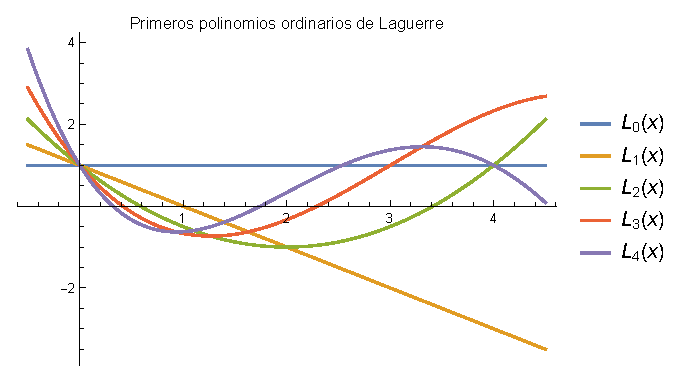
\includegraphics[scale=1.3]{Imagenes/Polinomios_Laguerre_01.eps}
    \caption{Gráfica con los primeros polinomios ordinarios de Laguerre.}
    \label{fig:grafica_Laguerre_01}
\end{figure}

A continuación se presenta una lista con los primeros polinomios asociados de Laguerre y una gráfica:
\begin{table}[H]
\centering
\large
\begin{tabular}{l l}
$L_{0}^{0} (x) = 1$ & $L_{0}^{2} = 2$  \\
$L_{1}^{0} (x) = - x + 1$ & $L_{1}^{2} = -6 \, x + 18$ \\
$L_{2}^{0} (x) = x^{2} - 4 x + 2$ & $L_{2}^{2} = 12 \, x^{2} - 96 \, x + 144$ \\
$L_{0}^{1} (x) = 1$ & $L_{0}^{3} = 6$ \\
$L_{1}^{1} (x) = -2x + 4$ & $L_{1}^{3} = -24 \, x + 96$ \\
\vdots 
\end{tabular}
\caption{Primeros polinomios asociados de Laguerre.}
\label{table:tabla_02}
\end{table}
\begin{figure}[H]
    \centering
    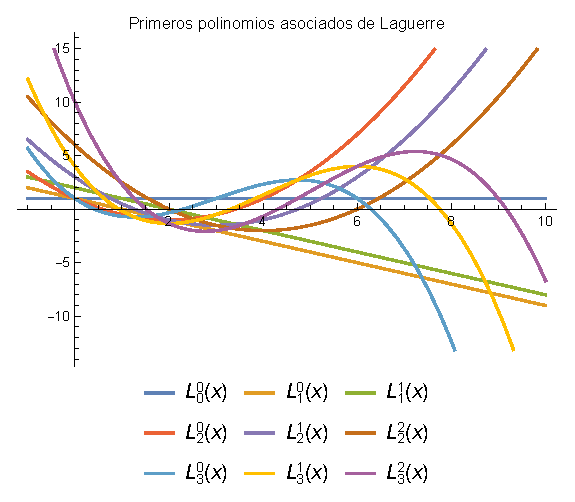
\includegraphics[scale=1.3]{Imagenes/Polinomios_Laguerre_02.eps}
    \caption{Gráfica con los primeros polinomios asociados de Laguerre.}
    \label{fig:grafica_Laguerre_02}
\end{figure}

Las funciones de onda normalizadas para el hidrógeno son:
\begin{align}
\setlength{\fboxsep}{3\fboxsep}\boxed{
\psi_{n \ell m} = \sqrt{\left(\dfrac{2}{n \, a} \right)^{3} \dfrac{(n - \ell - 1)}{2 \, n[(n + \ell)!]^{3}}} e^{-r/na} \; \left( \dfrac{2 \, r}{n \, a} \right)^{\ell} \; L_{n - \ell -1}^{2 \ell + 1} \left( \dfrac{2 \, r}{n \, a} \right) Y_{\ell}^{m} \, (\theta, \phi)}
\label{eq:ecuacion_04_89}
\end{align}

No se miran muy agradables, pero no se quejan, este es uno de los muy pocos sistemas realistas que se puede resolver del todo, de forma exacta. Como verá más adelante, son mutuamente ortogonales:
\begin{align}
\int \psi_{n \ell m}^{*} \psi_{\ptilde{n} \ptilde{\ell} \ptilde{m}} \, r^{2} \, \sin \theta \dd{r} \dd{\theta} \dd{\phi} =  \delta_{n \prime{n}} \delta_{\ell \delta{\ell}} \delta_{m \delta{m}}
\label{eq:ecuacion_04_90}
\end{align}

Esto se debe a la ortogonalidad de los armónicos esféricos y (para $n \neq n$) de que son las funciones propias de $H$ con distinto valor propio.
\par
Visualizar como tal las funciones de onda del hidrógeno no es fácil, a los químicos les agrada usar \enquote{gráficas de densidad}, en las cuales el nivel de brillo de la nube es proporcional a $\abs{\Psi}^{2}$, como se puede ver en la figura\footnote{Tomada con licencia de: https://commons.wikimedia.org/wiki/File:Hydrogen_Density_Plots.png  \href{https://commons.wikimedia.org/wiki/File:Hydrogen_Density_Plots.png}{Visita el sitio.}} :
\begin{figure}[H]
    \centering
    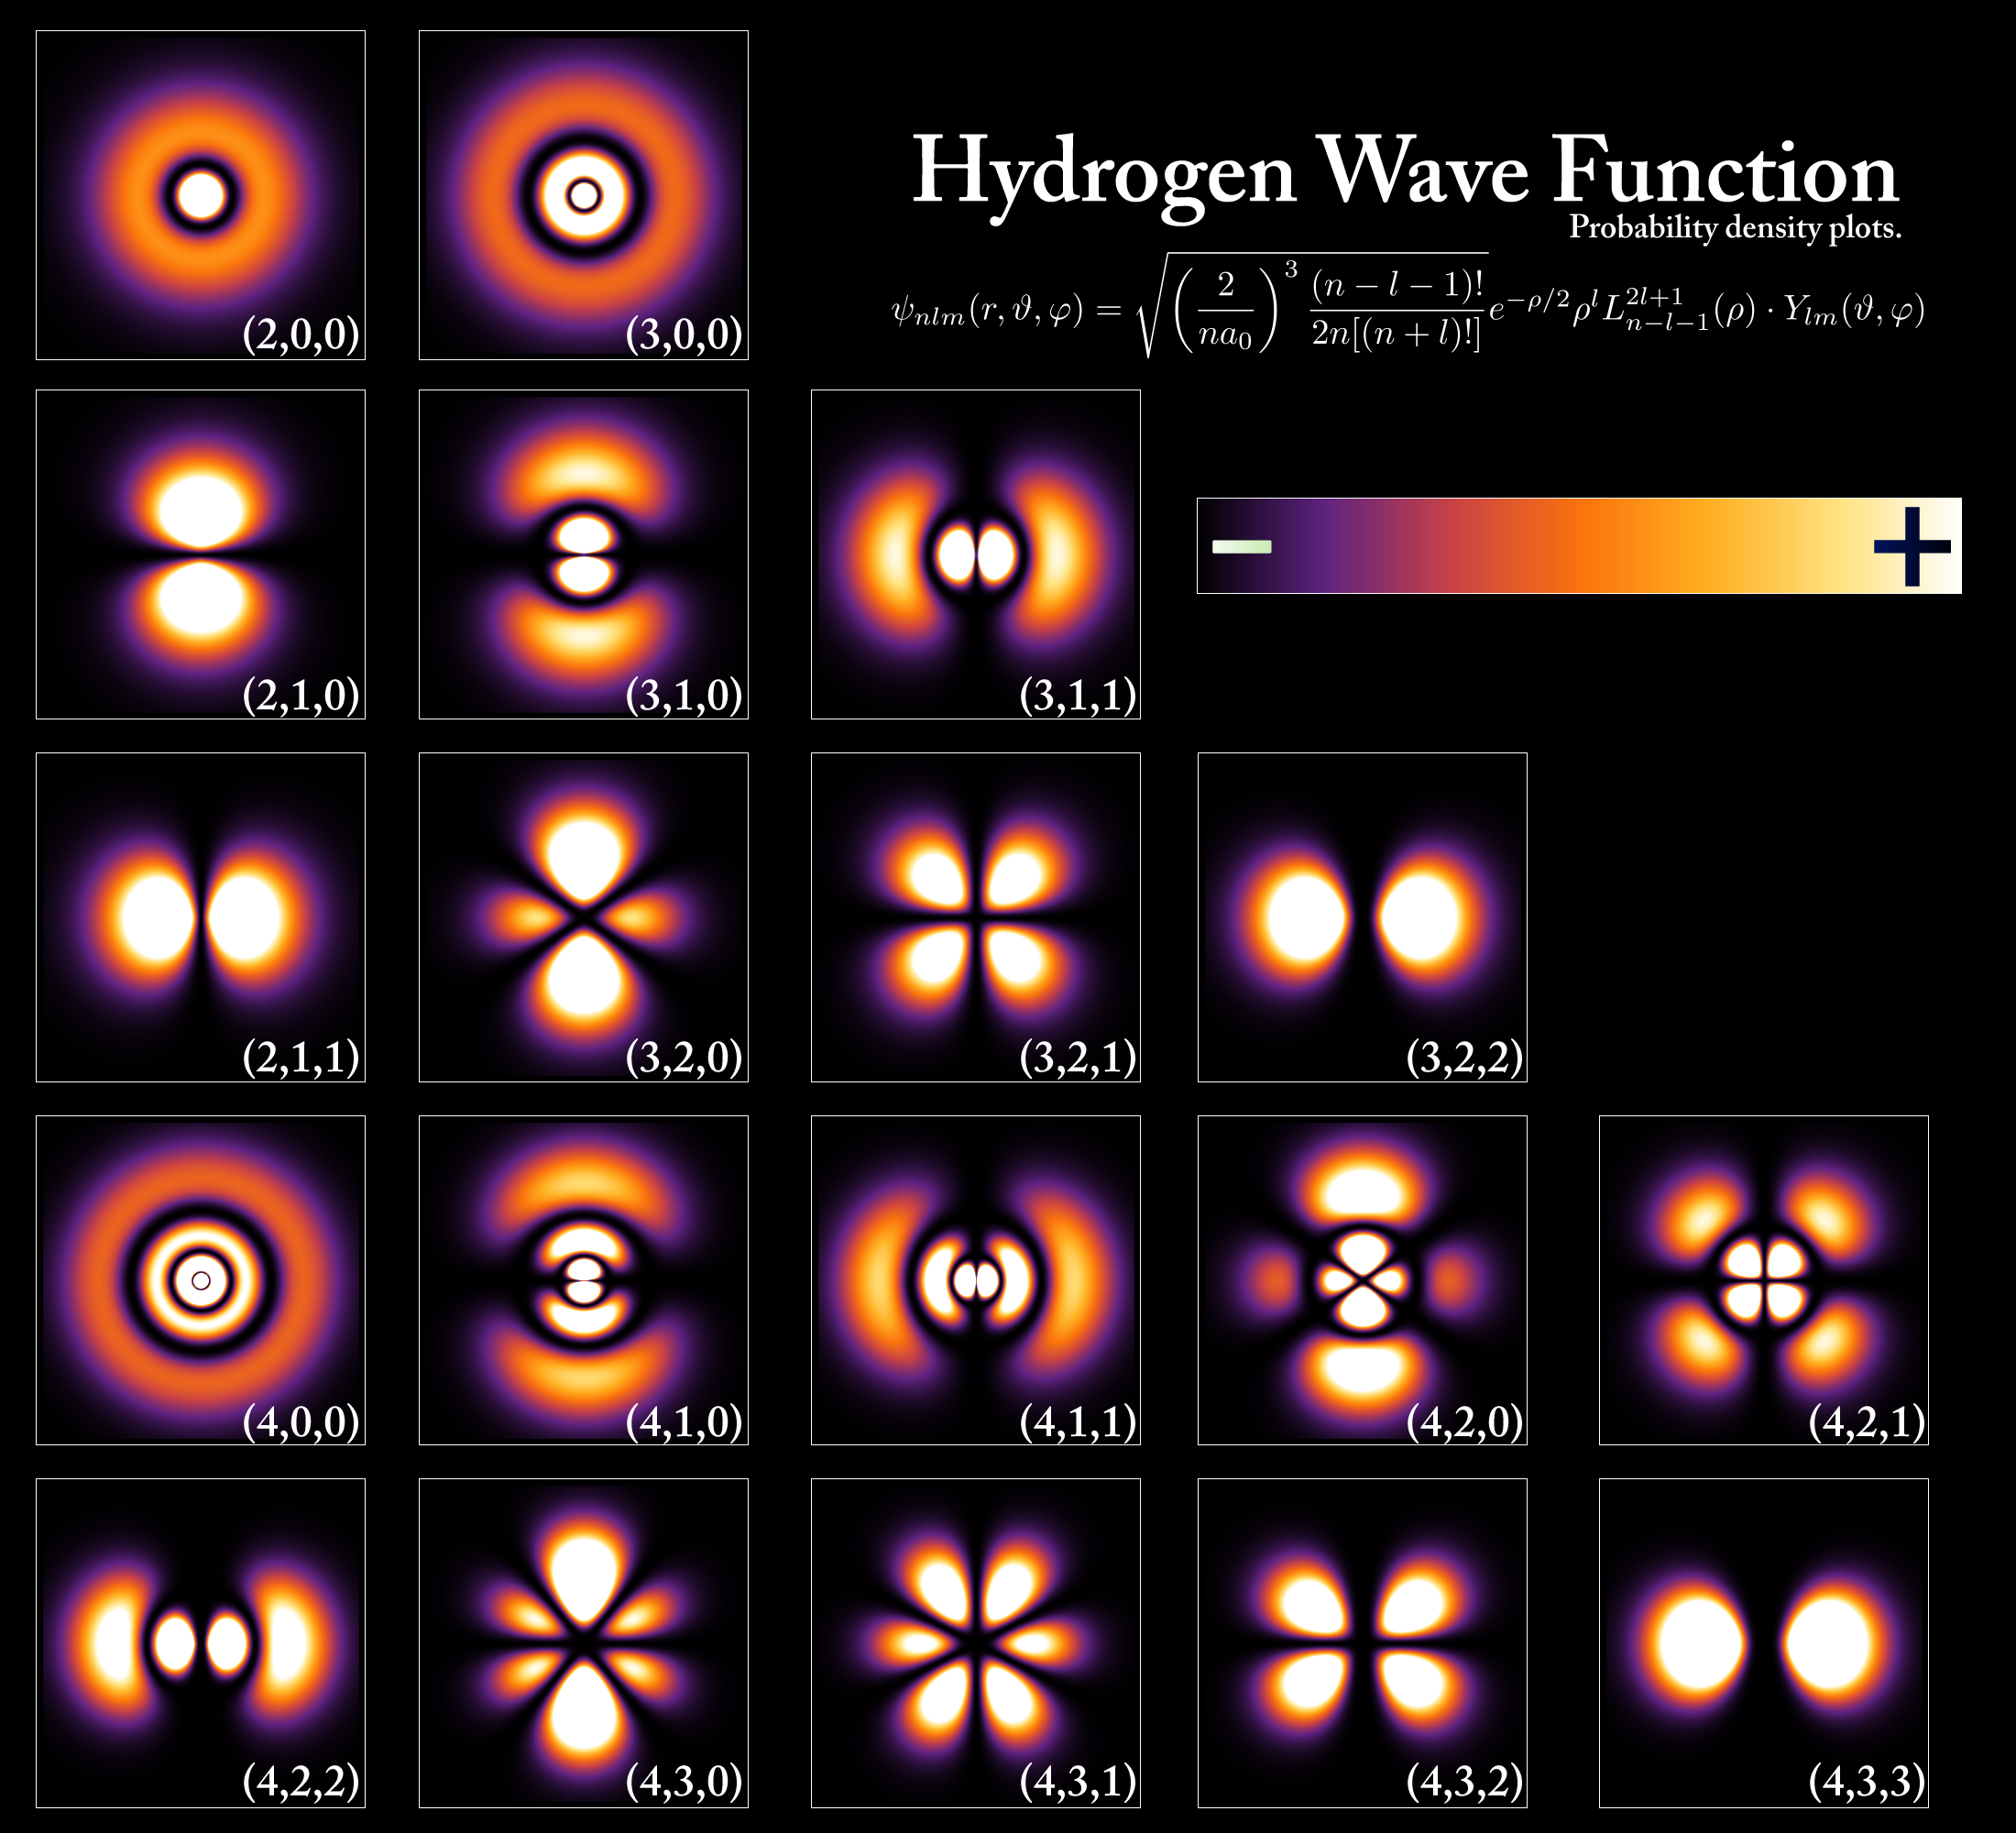
\includegraphics[scale=0.15]{Imagenes/Hydrogen_Density_Plots.png}
    \caption{Gráficas de densidad de estado para el hidrógeno}
\end{figure}

\subsection{Espectro del hidrógeno.}

En principio, si ponemos un átomo de hidrógeno en un estado estacionario $\Psi_{n \ell m}$, debe quedarse allí para siempre. Sin embargo, si \emph{perturbamos} ligeramente (por colisión con otro átomo, por ejemplo, o haciéndole incidir  luz en él), entonces el átomo puede experimentar una transición a otro estado estacionario mediante la absorción de la energía y pasarse a un estado de mayor energía o cediendo energía (normalmente en forma de radiación electromagnética) y moverse  hacia abajo.
\par
En la práctica este tipo de perturbaciones están siempre presentes; transiciones (o, como a veces se denominan \enquote{saltos cuánticos}) se producen constantemente, y el resultado es que un contenedor de hidrógeno emite luz (fotones), cuya energía corresponde a la diferencia de energía entre los estados inicial y final:
% \begin{align}
% E_{\gamma} = E_{i} - E_{f} = \SI{-13.6}{\electronvolt} \left( \dfrac{1}{n_{i}^{2}} - \dfrac{1}{n_{f}^{2}} \right)
% \label{eq:ecuacion_04_91}
% \end{align}
% de acuerdo con la fórmula de Planck, la energía de un fotón es proporcional a su frecuencia
% \begin{align}
% E_{\gamma} = h \, \nu
% \label{eq:ecuacion_04_92}
% \end{align}
% Mientras que la longitud de onda está dada por $\lambda = c / \nu)$, por tanto
% \begin{align}
% \dfrac{1}{\lambda} = R \left( \dfrac{1}{n_{f}^{2}} - \dfrac{1}{n_{i}^{2}} \right)
% \label{eq:ecuacion_04_93}
% \end{align}
% donde
% \begin{align}
% R = \dfrac{m}{4 \, \pi \, c \, \hbar} \left( \dfrac{e^{2}}{4 \, \pi \, \epsilon_{0}} \right)^{2} = \SI{1.097e7}{\per\metre}
% \label{eq:ecuacion_04_94}
% \end{align}
% a $R$ se le conoce como la \textbf{constante de Rydberg}, y la ec. (\ref{eq:ecuacion_04_93}) es la \textbf{fórmula Rydberg} para el espectro de hidrógeno. Fue descubierto empíricamente en el siglo XIX, y el mayor triunfo de la teoría de Bohr fue su capacidad para dar cuenta de este resultado y calcular $R$ en función de las constantes fundamentales de la naturaleza.
% \par
% Las transiciones al estado base ($n_{f}= 1$) se encuentran en el ultravioleta; son conocidas por los espectroscopistas como la \textbf{serie de Lyman}. Las transiciones al primer estado excitado ($n_{f}= 2$) se encuentran en la zona de región visible; conforman la \textbf{serie de Balmer}. Las transiciones a $n_{f} = 3$ (la \textbf{serie de Paschen}) están en el infrarrojo, y así sucesivamente (véase la figura \ref{fig:figura_espectro_H}). (A temperatura ambiente, la mayoría de los átomos de hidrógeno están en el estado base, para obtener el espectro de emisión, se deben elevar primero los diferentes estados excitados, por lo general esto se realiza haciendo pasar una chispa eléctrica a través del gas.)
% \begin{figure}[H]
%     \centering
%     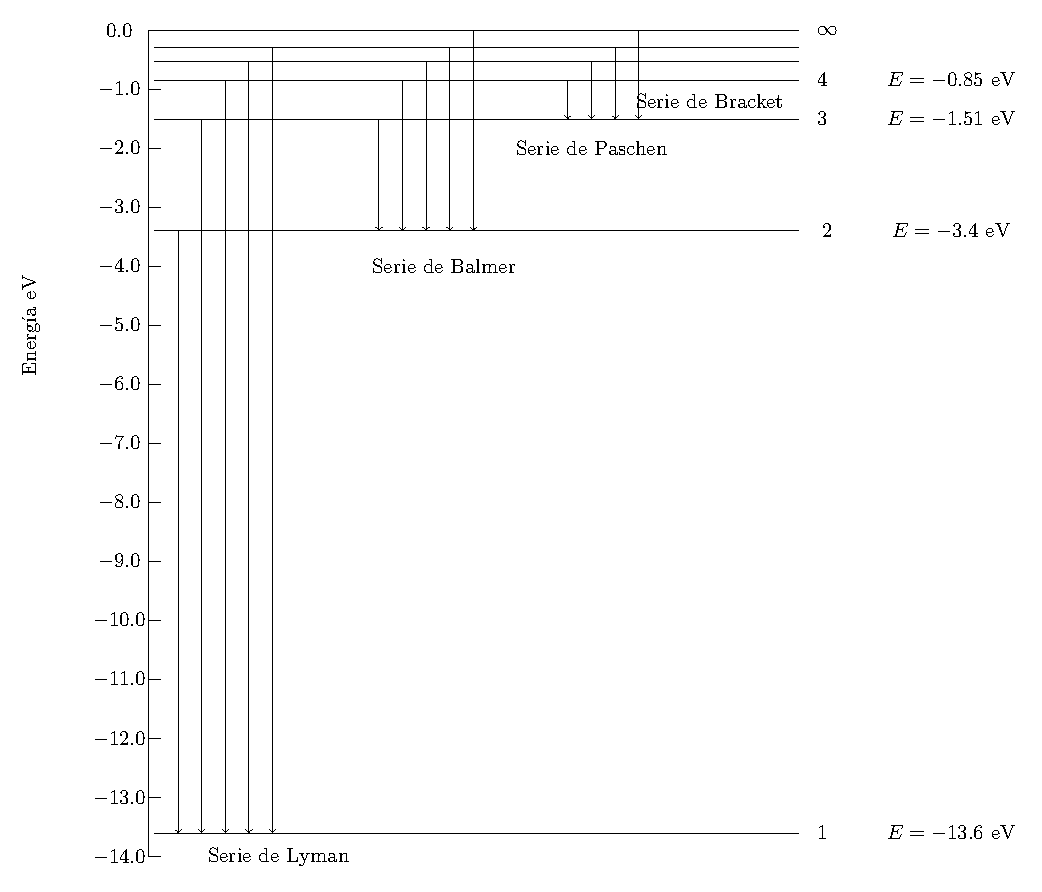
\includegraphics[scale=0.8]{Imagenes/espectrohidrogeno.eps}
%     \caption{Niveles de energía y transiciones en el espectro de hidrógeno.}
%     \label{fig:figura_espectro_H}
% \end{figure}


\end{document}